\documentclass{article}
\usepackage[utf8]{inputenc}
\usepackage{amsmath,amssymb,mathtools}
\usepackage{amsthm}
\usepackage{thmtools}
\usepackage{hyperref}
% `cleveref` has to be loaded after `hyperref`
\usepackage{cleveref}
\usepackage{stackengine}
\usepackage{minted}
\usepackage{tcolorbox}
\usepackage{multicol}
\usepackage{prftree}
\usepackage{fancyvrb}
\usepackage{csquotes}
\usepackage{appendix}
\usepackage{todonotes}

\newcommand{\traian}[1]{\todo[author=Traian]{#1}}
\newcommand{\jt}[1]{\todo[author=Jan]{#1}}

\title{Cartesian Reachability Logic: A Language-Independent Logic for Verifying $k$-Safety Properties}
\author{Jan Tu\v{s}il  \and Traian Florin Șerbănuță \and Xiaohong Chen
%\and Jan Obdrzalek
}
\date{\today}

\declaretheorem[]{example}
\declaretheorem[]{definition}
\declaretheorem[]{lemma}
\declaretheorem[]{theorem}
\declaretheorem[]{remark}

\newcommand{\K}{$\mathbb{K}$}
\newcommand{\RL}{\mathsf{RL}}
\newcommand{\ML}{\mathsf{ML}}
\newcommand{\CRL}{\mathsf{CRL}}
\newcommand{\FOL}{\mathsf{FOL}}
\newcommand{\FOLeq}{\FOL_{=}}
\newcommand{\Var}{\mathit{Var}}
\newcommand{\Tcfg}{\mathcal{T}_{\mathit{Cfg}}}
\newcommand{\Pattern}{\mathsf{Pattern}}

\newcommand\oast{\stackMath\mathbin{\stackinset{c}{0ex}{c}{0ex}{\ast}{\bigcirc}}}

\newenvironment{proofenv}
  {
    \VerbatimEnvironment\begin{tcolorbox}[colback=black!0!white] % 5 is the default
  }
  {
   \end{tcolorbox}
  }

\begin{document}

\maketitle

\section{Introduction}
Recent years have witnesssed an increased interest in formal verification of \emph{hyperproperties}.
A hyperproperty is a set of \emph{sets of} execution traces, with the following semantics:
a system $S$ (a set of traces) satisfies a hyperproperty $H$ iff $S \in H$.
Hyperproperties are strictly more expressive then properties; for example, many security policies
of interest are hyperproperties but not properties.

Techniques and tools for verifying hyperproperties of (finite-state) hardware \cite{CoenenFST19,FinkbeinerRS15},
as well as (infinite-state) software systems have been developed.
For verification of software systems in particular, \emph{Cartesian Hoare logic} (CHL, \cite{SousaD16}) extends Hoare logic
to reason about \emph{$k$-safety hyperproperties}
(a hyperproperty is a \emph{$k$-safety hyperproperty} if its violation can be witnessed
by a set of traces of size $k$).
However, it is not clear how to use these techniques with arbitrary programming languages,
since CHL is tied to a particular imperative language.

On the other hand, there have been recent developments in the are of \emph{language-independent} software verification.
\emph{Reachability logic} (RL) \cite{RosuS12oopsla,RosuSCM13lics,StefanescuCMMSR19}
is a
formalism for reasoning about partial correctness of software, in the spirit of Hoare logics.
Being implemented in the \K{} framework \cite{KVision},
its biggest advantage is that reachability logic is \emph{language independent}:
its proof system can be used unchanged to reason about programs in any language,
as long as the language has a formal semantics in RL.
Therefore, researchers no longer need to think about a particular language construct three times
(once for the operational semantics, once for axiomatic, and once for the correspondence);
additionally, a single researcher or a tool-builder does not need to understand both the precise (and often intricate)
semantics of a programming language, \emph{and} formal verification techniques,
which makes \emph{division of labour} possible.
Through \K{}, reachability logic has been used to build verifiers for real-world languages,
such as C (\cite{RVMatch}), Java (\cite{StefanescuPYLR16VerifiersForAll}), Javascript (\cite{StefanescuPYLR16VerifiersForAll}),
and EVM (\cite{KevmVerificationTool}).

Can we have the best of both worlds? We think it is possible.
In this paper we develop a logic named \emph{Cartesian Reachability logic (CRL)}, which properly extends reachability logic
to allow reasoning about $k$-safety hyperproperties. Simiarly to CHL, CRL has a sound
and relatively complete proof system. A major advantage of CRL against CHL is that it works with any language
for which RL works; that is, with any language which has a RL-based formal semantics.
However, CRL does \emph{not} extend CHL, because the two logics give different semantics to properties of nondeterministic programs;
despite this distinction, CRL extends CHL on the deterministic fragment of the CHL-supported language.
We elaborate on this relation in \Cref{sec:discussion}. 

The idea behind soundness and completeness of our approach is similar to the one of \cite{SousaD16} for CHL.
We define a language-agnostic equivalent of self-composition (\cite{BartheDR11}) and establish a relation
between CRL validity of the original and RL validity of the composed system.
Then we construct a proof system such that its proofs can be translated to ordinary RL proofs of the composed system
(for soundness),
but also such that it allows relatively high-level reasoning about \emph{circular behavior} and \emph{lock-step execution}
(for ease of verification and simplicity of invariants).
We draw our inspiration from the literature on language-independent verification of partial correctness
(\cite{RosuS12oopsla,RosuSCM13lics,StefanescuCMMSR19})
and program equivalence (\cite{CiobacaLRR16,CiobacaLRR14}).
Again, we elaborate on the similarities and differences in \Cref{sec:discussion}. 

\section{Preliminaries}

\subsection{($\mu$-free) Matching Logic}

We work with a variant of matching logic described in
\cite{StefanescuCMMSR19,RosuSCM13lics}.

\begin{definition}[Matching logic syntax and semantics]\label{def:matchinglogic}
We define the matching logic syntax and semantics as follows.
\begin{enumerate}
    \item A matching logic \emph{signature} $\mathbf{\Sigma} = (\Sigma, \mathit{Var})$ is a many-sorted algebraic signature $\Sigma$ together with a sort-wise infinite set of variables $\mathit{Var}$.
    \item Let $T_{\Sigma}(\mathit{Var})$ denote the free $\Sigma$-algebra of terms with variables 
          in $\mathit{Var}$.
          Let $T_{\Sigma, s}(\mathit{Var})$ denote the set of $\Sigma$-terms (with variables in $\mathit{Var})$ of sort $s$.
    \item Let $\mathcal{T}$ be a $\Sigma$-algebra, and $f$ be a symbol from $\Sigma$.
          We use the notation $\mathcal{T}_f$ to denote the interpretation of $f$ in $\mathcal{T}$.
    \item A function $\rho : \mathit{Var} \to \mathcal{T}$, where $\mathcal{T}$ is a $\Sigma$-algebra,
          extends uniquely (in the usual way) to a $\Sigma$-algebra morphism
          $\rho : T_{\Sigma}(\mathit{Var}) \to \mathcal{T}$.
    \item The set of \emph{nullary predicate symbols} $P_\epsilon((\Sigma, \mathit{Var}))$
          (or just $P_\epsilon$ if $(\Sigma, \mathit{Var})$ is known from the context) is
          defined to contain exactly terms $\phi \in T_{\Sigma, s}(\mathit{Var})$.
    \item A matching logic $(\Sigma, \mathit{Var})$-formula (aka $(\Sigma, \mathit{Var})$-\emph{pattern})
          of sort $s$
          is a $(\Sigma, P_\epsilon)-\FOLeq$ formula (that is, a $\FOLeq$ formula where function symbols are
          exactly symbols from $\Sigma$, and where nullary predicate symbols are exactly
          terms $\phi \in T_{\Sigma, s}(\mathit{Var})$, without any $k$-ary predicate symbols for $k > 0$).
          We let $\Pattern(\mathbf{\Sigma})$ (or just $\Pattern$ when $\mathbf{\Sigma}$ is known from the context)
          denote the set of all $\mathbf{\Sigma}$-patterns.
    \item Let $\mathit{FV}(\varphi)$ denote the set of all free variables of $\varphi$.
    \item A matching logic pattern is \emph{structureless} if it contains
          no terms $\phi \in T_{\Sigma, s}(\mathit{Var})$ used as predicates.
    \item A \emph{constrained term} is a pattern of the form $\phi \land P$,
          where $\phi \in T_{\Sigma, s}(\mathit{Var})$ and $P$ a structureless pattern.
    \item A matching logic $\Sigma$-\emph{model} $\mathcal{T}$ is a $\Sigma$-algebra with non-empty carrier sets.
    \item A matching logic \emph{semantics} is given by means of
          the satisfaction relation $\vDash_{\ML}$ between a matching logic $\Sigma$-model,
          a model element, and a valuation,
          defined inductively as
          \begin{itemize}
              \item $(\mathcal{T}, \gamma, \rho) \vDash \phi$ iff $\gamma = \rho(\pi)$, where $\phi \in T_{\Sigma, s}(\mathit{Var})$;
              \item $(\mathcal{T}, \gamma, \rho) \vDash \varphi_1 \land \varphi_2$ iff
                $(\mathcal{T}, \gamma, \rho) \vDash \varphi_1$ and
                $(\mathcal{T}, \gamma, \rho) \vDash \varphi_2$;
              \item $(\mathcal{T}, \gamma, \rho) \vDash \neg \varphi$ iff
                $(\mathcal{T}, \gamma, \rho) \not\vDash \varphi$;
              \item $(\mathcal{T}, \gamma, \rho) \vDash \exists x : s.\, \varphi$ iff
                $(\mathcal{T}, \gamma, \rho^\prime) \vDash \varphi$ for some $\rho^\prime$ such that
                $\rho^\prime(y) = \rho(y)$ for all $y \in \mathit{Var} \setminus \{ x \}$
                and $\rho^\prime(x) \in \mathcal{T}_s$;
          \end{itemize}
          
\end{enumerate}

\end{definition}

Validity of a structureless pattern does not depend on the selected model element.
\begin{lemma}\label{lem:structurelessSemantics}
Let $\mathcal{T}$ be a matching logic $\Sigma$-model, $\gamma,\gamma^\prime \in \mathcal{T}$ model elements,
and $\rho$ a $\mathcal{T}$-valuation. Then for any structureless pattern $P$,
\begin{equation*}
    (\mathcal{T}, \gamma, \rho) \vDash P \iff (\mathcal{T}, \gamma^\prime, \rho) \vDash P \, .
\end{equation*}
Therefore, when $P$ is structureless, we may sometimes write $(\mathcal{T}, \rho) \vDash P$ to mean that 
$(\mathcal{T}, \gamma, \rho) \vDash P$ for \emph{some} $\gamma \in \mathcal{T}$.
\end{lemma}

Also, validity of any pattern does not depend on those variables which the pattern does not mention.
\begin{lemma}\label{lem:unusedVariables}
    Let $\mathcal{T}$ be a matching logic model, $\gamma$ an element of this model,
    and $\varphi$ a pattern.
    Then for any two $\mathcal{T}$-valuations $\rho,\rho^\prime$
    satisfying $\rho^\prime(y) = \rho(y)$ for any $y \in \mathit{FV}(\varphi)$,
    \begin{equation*}
        (\mathcal{T}, \gamma, \rho) \vDash \varphi \iff (\mathcal{T}, \gamma, \rho^\prime) \vDash \varphi \, .
    \end{equation*}
\end{lemma}
\begin{proof}
Admitted.
\end{proof}


\subsection{One-path Reachability Logic}



\begin{definition}[\cite{StefanescuCMMSR19,RosuS12oopsla}]\label{def:basics}
We define reachability-logic signatures, rules, and systems as follows.
\begin{enumerate}
    \item A reachability-logic \emph{signature} is a pair $(\mathbf{\Sigma}, \mathit{Cfg})$,
          where $\mathbf{\Sigma}$ is a matching logic signature and $\mathit{Cfg}$ is a sort from $\mathbf{\Sigma}$.
          
    \item A \emph{one-path reachability rule} over reachability logic signature $(\mathbf{\Sigma}, \mathit{Cfg})$        is a pair $\varphi \Rightarrow^\exists \varphi^\prime$,
          where $\varphi$ and $\varphi^\prime$
          are $\mathbf{\Sigma}$-patterns (which can have free variables) of sort $\mathit{Cfg}$.
          
    \item A \emph{reachability system} over a reachability-logic signature $((\Sigma, \mathit{Var}), \mathit{Cfg})$
          is a pair $\mathcal{S} = (\mathcal{T}, S)$, where $\mathcal{T}$ is a $\Sigma$-algebra
          and $S$ is a set of reachability rules over $((\Sigma, \mathit{Var}), \mathit{Cfg})$.
          
    \item A rule $\varphi \Rightarrow^\exists \varphi^\prime$ over $((\Sigma, \mathit{Var}), \mathit{Cfg})$
          is \emph{weakly well-defined}
          with respect to $\Sigma$-algebra $\mathcal{T}$
          iff
          for any $\gamma \in \Tcfg$ and $\rho : \Var \to \mathcal{T}$
          with $(\gamma, \rho) \vDash \varphi$,
          there exists $\gamma^\prime \in \Tcfg$ with $(\gamma^\prime , \rho) \vDash \varphi^\prime$.
          
    \item A reachability system $\mathcal{S}$ is \emph{weakly well-defined} iff each its rule is weakly     
          well-defined.
          
    \item A reachability system $\mathcal{S} = (\mathcal{T}, S)$ over $((\Sigma, \mathit{Var}), \mathit{Cfg})$ induces
          a \emph{transition system} \\
          $(\Tcfg , \Rightarrow_{\mathcal{S}})$,
          where $\gamma \Rightarrow_{\mathcal{S}} \gamma^\prime$
          for $\gamma, \gamma^\prime \in \Tcfg$
          iff there is some rule \\ $\varphi \Rightarrow^\exists \varphi^\prime \in S$
          and some valuation $\rho : \Var \to \mathcal{T}$ with $(\gamma, \rho) \vDash \varphi$
          and $(\gamma^\prime , \rho) \vDash \varphi^\prime$.

    \item A reachability system $(\mathcal{T}, S)$ is \emph{deterministic} iff the induced transition system
          is deterministic.
          
    \item A reachability system $(\mathcal{T}, S)$ is \emph{$\epsilon$-free}
          iff for any two configurations $\sigma, \sigma^\prime \in \mathcal{T}_{\mathit{Cfg}}$, if
          $\sigma \Rightarrow_{\mathcal{S}} \sigma^\prime$, then $\sigma \not = \sigma^\prime$.

    \item A configuration $\gamma \in \Tcfg$ \emph{terminates} in $(\Tcfg , \Rightarrow_{\mathcal{S}})$
          iff there is no infinite $\Rightarrow_{\mathcal{S}})$-sequence starting with $\gamma$.
          
    \item A \emph{$\Rightarrow_{\mathcal{S}}$-path} is a finite
          sequence $\gamma_0 \Rightarrow_{\mathcal{S}} \gamma_1 \Rightarrow_{\mathcal{S}} \ldots
          \Rightarrow_{\mathcal{S}} \gamma_n$
          with $\gamma_0,\ldots,\gamma_n \in \Tcfg$.
          
    \item A $\Rightarrow_{\mathcal{S}}$-path is \emph{complete}
          iff it is not a strict prefix of any
          other $\Rightarrow_{\mathcal{S}}$-path.

    \item \label{def:oprlSemantics}
          A one-path reachability rule $\varphi \Rightarrow^\exists \varphi^\prime$ is \emph{satisfied}
          in a reachability system $\mathcal{S} = (\mathcal{T}, S)$,
          written $\mathcal{S} \vDash_\RL \varphi \Rightarrow^\exists \varphi^\prime$,
          iff for every $\gamma \in \Tcfg$
          such that $\gamma$ terminates in $(\Tcfg, \Rightarrow_{\mathcal{S}})$
          and for any valuation $\rho : \Var \to \mathcal{T}$
          such that $(\gamma, \rho) \vDash \varphi$,
          there exists some $\gamma^\prime \in \Tcfg$
          such that
          $\gamma \Rightarrow^{*}_{\mathcal{S}} \gamma^\prime$
          and $(\gamma^\prime, \rho) \vDash \varphi^\prime$.
          
          
%    \item An \emph{all-path reachability rule} is a pair
%        $\varphi \Rightarrow^\forall \varphi^\prime$ of patterns $\varphi$ and $\varphi^\prime$.
%    
%    \item \label{def:aprlSemantics}
%          An all-path reachability rule $\varphi \Rightarrow^\forall \varphi^\prime$ is \emph{satisfied},
%          written $\mathcal{S} \vDash_\RL \varphi \Rightarrow^\forall \varphi^\prime$,
%          iff for all complete $\Rightarrow_{\mathcal{S}}$-paths $\tau$
%          starting with $\gamma \in \Tcfg$ and for all $\rho : \Var \to \mathcal{T}$
%          such that $(\gamma, \rho) \vDash \varphi$,
%          there exists some $\gamma^\prime \in \tau$
%          such that $(\gamma^\prime, \rho) \vDash \varphi^\prime$.
\end{enumerate}

%\begin{figure}
%    \centering
%    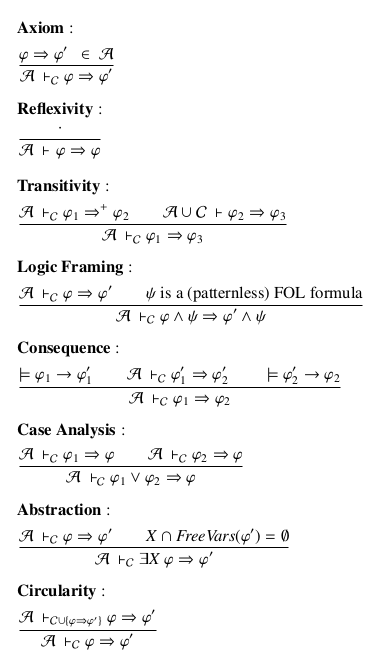
\includegraphics[width=0.5\textwidth]{img/onepath-rl.png}
%    \caption{One-path reachability-logic proof system.
%    The use of $\Rightarrow^+$ in sequent means that it was derived without Reflexivity.
%    TODO retypeset}
%    \label{fig:RLproofsystem}
%\end{figure}

We have RL sequents of the shape
$\mathcal{T}, A, C \vdash_\RL \varphi \Rightarrow^\exists \varphi^\prime$.

\end{definition}

\begin{remark}\label{rem:shapeOfReachabilityRules}
For simplicity, we restrict the class of reachability systems we work with to those whose reachability rules
have only disjunctions of constrained terms. That is, we assume all rules have the shape
\begin{equation*}
    \exists \vec{X}.\, \bigvee_{i=1}^{m} (\phi_i \land P_i) \Rightarrow^\exists \exists \vec{Y}.\, \bigvee_{j=1}^{n} (\phi^\prime_j \land P^\prime_j) \, .
\end{equation*}
\end{remark}

\begin{remark}\label{rem:noEmptySteps}
We work only with $\epsilon$-free reachability systems.
\end{remark}

\section{Cartesian Reachability Logic}
Cartesian reachability logic is an extension of (one-path) reachability logic.

\begin{definition}[One-Path Cartesian Reachability Rule]\label{def:opCRLsemantics}
    We define syntax and semantics of cartesian reachability rules as follows.
\begin{itemize}
    \item 
        A One-Path Cartesian reachability rule of arity $k$ has the shape
        \begin{equation*}
        \exists \vec{X}.\, (\varphi_1,\ldots,\varphi_k) \land \varphi \Rightarrow^{c\exists} \exists \vec{Y}.\, (\psi_1,\ldots,\psi_k) \land \psi \, ,
        \end{equation*}
        where $\varphi, \psi$ are structureless patterns and $\varphi_j, \psi_j$ for any $j \in \{ 1, \ldots, k \}$ are
        existentially quantified\jt{Check whether we need that.} disjunctions of constrained terms.
    \item 
    A One-Path Cartesian reachability rule
    \begin{equation*}
     \exists \vec{X}.\, (\varphi_1,\ldots,\varphi_k) \land \varphi
     \Rightarrow^{c\exists} \exists \vec{Y}.\, (\psi_1,\ldots,\psi_k) \land \psi   
    \end{equation*}
    is \emph{valid} in a reachability system $\mathcal{S} = (\mathcal{T}, S)$,
    written
    \begin{equation*}
        \mathcal{S} \vDash_\CRL \exists \vec{X}.\, (\varphi_1,\ldots,\varphi_k) \land \varphi
     \Rightarrow^{c\exists} \exists \vec{Y}.\, (\psi_1,\ldots,\psi_k) \land \psi \, ,
    \end{equation*}
    iff for all configurations $\gamma_1,\ldots,\gamma_k \in \Tcfg$
    which terminate in $(\Tcfg, \Rightarrow_{\mathcal{S}})$
    and any two $\mathcal{T}$-valuation $\rho,\rho^\prime$
    satisfying $\rho(v) = \rho^\prime(v)$ for any $v \in \mathit{Var} \setminus (\vec{X} \cup \vec{Y})$,
    whenever $(\gamma_1,\rho) \vDash \varphi_1 \land \varphi$ and \ldots
    and $(\gamma_k,\rho) \vDash \varphi_k \land \varphi$,
    then there exist configurations $\gamma_1^\prime,\ldots,\gamma_k^\prime \in \Tcfg$
    such that $\gamma_1 \Rightarrow^{*}_{\mathcal{S}} \gamma_1^\prime$  
    and \ldots and $\gamma_k \Rightarrow^{*}_{\mathcal{S}} \gamma_k^\prime$,
    and
    $(\gamma_1^\prime,\rho^\prime) \vDash \psi_1 \land \psi$ and \ldots and $(\gamma_k^\prime, \rho^\prime) \vDash \psi_k \land \psi$.
\end{itemize}
\end{definition}

% TODO remark that this is not the same as k "normal" reachability rules.
% An example (monotonicity from the file)

\begin{remark}
\Cref{def:opCRLsemantics} extends \Cref{def:oprlSemantics} of \Cref{def:basics}:
if we fix $k=1$, then
\begin{align*}
    (\mathcal{T}, S) \vDash_\CRL
    (\varphi_1) \land \top  \Rightarrow^{c\exists}
    (\psi_1) \land \top
    \iff
    (\mathcal{T}, S) \vDash_\RL \varphi_1 \Rightarrow^{\exists} \psi_1 \, .
\end{align*}
\end{remark}

%\begin{definition}[All-Path Cartesian Reachability Rule]\label{def:apCRLsemantics}
%An all-path Cartesian reachability rule
%$(\varphi_1,\ldots,\varphi_k) \land \varphi \Rightarrow^{c\forall} (\psi_1,\ldots,\psi_k) \land \psi$
%of arity $k$
%is \emph{valid} in a reachability system $\mathcal{S} = (\mathcal{T}, S)$,
%written
%$\mathcal{S} \vDash_\CRL (\varphi_1,\ldots,\varphi_k) \land \varphi \Rightarrow^{c\forall}
%(\psi_1,\ldots,\psi_k) \land \psi$,
%iff for all configurations $\sigma_1,\ldots,\sigma_k \in \Tcfg$ \traian{Why $\sigma$ instead of $\gamma$?}
%and any $\mathcal{T}$-valuation $\rho$,
%whenever $(\sigma_1, \rho) \vDash \varphi_1 \land \varphi$ and \ldots
%and $(\sigma_k, \rho) \vDash \varphi_k \land \varphi$,
%then for every $k$-tuple of complete paths $(\pi_1, \ldots, \pi_k)$
%such that
%$\sigma_1 = \pi_1(0) \land \ldots \land \sigma_k = \pi_k(0)$,
%there exist indices $i_1, \ldots, i_k$ such that
%$(\pi_1(i_1), \rho) \vDash \varphi_1 \land \psi$ and \ldots and $(\pi_k(i_k), \rho) \vDash \varphi_k \land \psi$.
%\end{definition}

\begin{definition}\label{def:starextension}
We translate a language semantics into a semantics for lists of configurations as follows.
\begin{enumerate}
    \item Let $((\Sigma, \mathit{Var}), \mathit{Cfg})$ be a reachability-logic signature.
          Then $((\Sigma, \mathit{Var}^*), \mathit{Cfg})^*$ = $((\Sigma^*, \mathit{Var}^*), \mathit{Cfg}^*)$,
          where
          \begin{enumerate}
              \item $\Sigma^* = \Sigma \cup \{ \mathit{cfgitem}, \mathit{cfgconcat}, \mathit{cfgheat}, \mathit{cfgnil} \}$
              \item $\mathit{Cfg}^*$ is a fresh sort (representing the sort of lists of configurations);
              \item $\mathit{Var}^* = \mathit{Var} \cup \mathit{Var}_{\mathit{Cfg}^*}$,
              where $\mathit{Var}_{\mathit{Cfg}^*}$ is an infinite set of variables of sort $\mathit{Cfg}^*$,
              distinct from varibles in $\mathit{Var}$;
              \item $\mathit{cfgitem}$ a fresh symbol of sort $\mathit{Cfg} \to \mathit{Cfg}^*$;
              \item $\mathit{cfgnil}$ a fresh symbol of sort $\mathit{Cfg}^*$;
              \item $\mathit{cfgconcat}$ a fresh symbol of sort $\mathit{Cfg}^* \times \mathit{Cfg}^* \to \mathit{Cfg}^*$; and
              \item $\mathit{cfgheat}$ is a fresh symbol of sort $\mathit{Cfg}^* \times \mathit{Cfg} \times \mathit{Cfg}^* \to \mathit{Cfg}^*$.
          \end{enumerate}
    \item Let $S$ be a set of reachability rules over $(\mathbf{\Sigma}, \mathit{Cfg})$.
          We generate a set of reachability rules $S^*$ over $(\mathbf{\Sigma}, \mathit{Cfg})^*$
          by
          \begin{enumerate}
              \item defining a function $\mathit{heat} : \mathit{Var} \times \Pattern \times \mathit{Var} \to \Pattern$ by
              \begin{align*}
                  \mathit{heat}(L, \exists \vec{X}.\, \bigvee_{i=1}^{m} (\phi_i \land P_i), R)
                  = \exists \vec{X}.\, \bigvee_{i=1}^{m} ( \mathit{cfgheat(L, \phi_i, R)} \land P_i)
              \end{align*}
              \item setting
              \begin{align*}
              S^* = \{ \mathit{heat}(L, \varphi, R) \Rightarrow^\exists \mathit{heat}(L, \varphi^\prime, R)
              \mid  ( \varphi \Rightarrow^\exists \varphi^\prime ) \in S \} \, ,
            \end{align*}
                          where $L,R$ are distinct fresh variables (not occurring in any rule in $S$).
          \end{enumerate}
    \item Let $(\Sigma, \mathit{Var})$ be a matching logic signature, and let $\mathcal{T}$ be a configuration model; that is, a $\Sigma$-algebra.
          We generate a $\Sigma^*$-algebra $\mathcal{T}*$, which interprets all sorts and symbols from
          $\Sigma$ as in $\mathcal{T}$, and in addition interprets
          \begin{enumerate}
              \item the sort $\mathit{Cfg}*$ as the set of all finite lists
              $[c_1;\ldots;c_n]$ for $n \in \mathbb{N}$, where $c_i$ is an element of sort $\mathit{Cfg}$
              for any $0 \leq i \leq n$;
              \item the symbol $\mathit{cfgitem}$ as the function $\lambda c.\, [c]$;
              \item the symbol $\mathit{cfgnil}$ as the empty list ($[]$);
              \item the symbol $\mathit{cfgconcat}$ as the function $\lambda l_1,l_2.\, l_1 \texttt{++} l_2$,
                where $\texttt{++}$ is list concatenation; and
              \item the symbol $\mathit{cfgheat}$ as the function
                $\lambda l_1, c, l_2.\, l_1 \texttt{++} [c] \texttt{++} l_2$.
          \end{enumerate}

    \item Let $(\Sigma, \mathit{Var})$ be a matching logic signature, let $\mathcal{T}$ be a configuration model,
        and let $\rho$ be a $\mathcal{T}$-valuation.
        We define a $\mathcal{T}^*$-valuation $\rho^*$ by letting $\rho^*(v) = \rho(v)$ for any $v \in \mathit{Var}$,
        and letting $\rho^*(v) = a$, where $a$ is some arbitrary element of sort $\mathit{Cfg}^*$, for
        any variable $v$ of sort $\mathit{Cfg}^*$.
          
    \item Let $\mathcal{S} = (\mathcal{T}, S)$ be a reachability system over $(\Sigma, \mathit{Cfg})$.
          We generate a reachability system $\mathcal{S}^*$ over $(\Sigma, \mathit{Cfg})^*$
          by setting $\mathcal{S}^* = (\mathcal{T}^*, S^*)$.
\end{enumerate}
\end{definition}

\begin{lemma}\label{lem:rhoStarOfPi}
    Let $(\Sigma, \mathit{Var})$ be a matching logic signature, $\mathcal{T}$ be a configuration model,
    and $\rho$ be a $\mathcal{T}$-valuation. Then for any basic $(\Sigma, \mathit{Var})$-pattern $\pi$,
    \begin{equation}
        \rho^*(\pi) = \rho(\pi) \, .
    \end{equation}
\end{lemma}

\begin{lemma}\label{lem:starConservative}
    The star extension on matching logic models is conservative, in the following sense.
    For any $\Sigma$-model $\mathcal{T}$, any $\mathcal{T}$-valuation $\rho$,
    any $\Sigma$-sort $s$,
    any $\gamma \in \mathcal{T}_s$,
    and any matching logic $s$-pattern $\varphi$,
    \begin{equation*}
        (\mathcal{T}, \gamma, \rho) \vDash \varphi \iff (\mathcal{T}^*, \gamma, \rho^*) \vDash \varphi
    \end{equation*}
\end{lemma}

\begin{lemma}\label{lem:compositeStep}
    Let $\mathcal{S} = (\mathcal{T}, S)$ be a reachability system over $(\Sigma, \mathit{Cfg})$.
    For any $k \geq 1$, any configurations $c_1,\ldots,c_k, c^\prime \in \Tcfg$, and any $1 \leq i \leq k$,
    we have
    \begin{equation*}
        c_i \Rightarrow_{\mathcal{S}} c^\prime
                    \iff
        [c_1,\ldots,c_k] \Rightarrow_{\mathcal{S}^*} [c_1, \ldots, c_{i-1}, c^\prime, c_{i+1}, \ldots, c_k]
    \end{equation*}
\end{lemma}


\begin{definition}
We define $\mathit{mkList}$, $\mathit{mergePatterns}$, and $\mathit{flatten}$ as follows:
\begin{enumerate}
    \item $\mathit{mkList}(\phi) = \mathit{cfgitem}(\phi)$
    \item $\mathit{mkList}(\phi_1, \ldots, \phi_k) = \mathit{cfgconcat}(\mathit{cfgitem}(\phi), \mathit{mkList}(\phi_2, \ldots, \phi_k))$ for $k > 1$
    \item
    \begin{align*}
     & \mathit{mergePatterns}(\exists \vec{X_1}.\, \bigvee_{i_{1}=1}^{m_1} (\phi_{i_1} \land P_{i_1}),
     \ldots, \exists \vec{X_n}.\, \bigvee_{i_{n}=1}^{m_n} (\phi_{i_n} \land P_{i_n}))
     \\ & = \exists \vec{X_1}\ldots\vec{X_n}.\, \bigvee_{i_{1}=1}^{m_1} \ldots \bigvee_{i_{n}=1}^{m_n}
       (\mathit{mkList}(\phi_{1, i_1}, \ldots, \phi_{n, i_n}) \land (P_{1, i_1} \land \ldots \land P_{n, i_n}))
    \end{align*}
    \item
        \begin{align*}
            \mathit{constrain}(P, \exists \vec{X^\prime} .\,
            \bigvee_{i=1}^{m} (\phi^\prime_i \land P^\prime_i))
            = (\exists \vec{X^\prime}.\, \bigvee_{i=1}^{m}(\phi^\prime_i \land (P^\prime_i \land P))
    \end{align*}
    (we assume that $\alpha$-renaming of (free) variables of $P$ happens implicitly \jt{?});
    \item
        \begin{align*}
            & \mathit{flatten}(\exists \vec{X}.\, (\varphi_1, \ldots, \varphi_k) \land P)
            = \exists \vec{X}.\, \mathit{constrain}(P, \mathit{mergePatterns}(\varphi_1, \ldots, \varphi_k))
    \end{align*}
    \item $\mathit{flatten}^\exists(\Psi, \Psi^\prime) = \mathit{flatten}(\Psi) \Rightarrow^\exists \mathit{flatten}(\Psi^\prime)$
    \item $\mathit{flatten}^\exists(A, \Psi^\prime) = \{ \mathit{flatten}^\exists(\Psi, \Psi^\prime) \mid \Psi \in A \}$, where $A$ is a set.
\end{enumerate}
\end{definition}

\begin{theorem}\label{thm:correspondence}
\begin{equation*}
\mathcal{S} \vDash_{\CRL} \Psi \Rightarrow^{c\exists} \Psi^\prime \iff \mathcal{S}^* \vDash_\RL \mathit{flatten}^\exists(\Psi, \Psi^\prime)
\end{equation*}
\end{theorem}

\section{Proof System}

The proof system derives claims of the shape
$\mathcal{S}, \vdash_\CRL \Phi \Downarrow_{C,E} \Psi$,
where $\Phi$,$\Psi$ are of the shape
$\exists \vec{X}.\, (\varphi_1, \ldots, \varphi_k) \land P$,
where $P$ is a structureless FOL formula
and every $\varphi_i$ has the structure of
$\exists x_1,\ldots,x_n. (\phi_1 \land P_1) \lor \ldots (\phi_m \land P_m)$.
The idea is that $P$ is the part of the claim that relates variables from different components.
Initially, the proof starts with the claim
$\mathcal{S} \vdash_\CRL \Phi \Downarrow_{\emptyset, \emptyset} \Psi$.


\begin{figure}
    \centering
    \begin{align*}
    & \prftree[l]{Reflexivity}{\mathcal{S} \vdash_\CRL \Psi \Downarrow_{\emptyset,E} \Psi}
    \end{align*}
    \begin{align*}
    & \prftree[l]{Axiom}{\Psi \in E}{\mathcal{S} \vdash_\CRL \Psi \Downarrow_{C,E} \Psi^\prime}
    \end{align*}
    \begin{align*}
    & \prftree[l]{Reduce}
      {(\mathcal{T}^*, S^* \cup \mathit{flatten}^\exists(E, \Psi^\prime)), \emptyset \vdash_\RL
        \mathit{flatten}^\exists(\Psi, \Psi^\prime) }
      {(\mathcal{T}, S) \vdash_\CRL \Psi \Downarrow_{C,E} \Psi^\prime}
    \end{align*}
    \begin{align*}
    & \prftree[l]{Case}
    { \prfStackPremises
      {\mathcal{S} \vdash_\CRL (\varphi_1, \ldots, \varphi_{i-1}, \varphi_i, \varphi_{i+1}, \ldots, \varphi_k) \land P^\prime \Downarrow_{C, E} \Psi^\prime }
      {\mathcal{S} \vdash_\CRL (\varphi_1, \ldots, \varphi_{i-1}, \psi_i, \varphi_{i+1}, \ldots, \varphi_k) \land P^\prime \Downarrow_{C, E} \Psi^\prime }
    }
    {\mathcal{S} \vdash_\CRL (\varphi_1, \ldots, \varphi_{i-1}, (\varphi_i \lor \psi_i), \varphi_{i+1}, \ldots, \varphi_k) \land P^\prime \Downarrow_{C, E} \Psi^\prime}
    \end{align*}
    \begin{align*}
    & \prftree[l]{Step}
    { \prfStackPremises
       {\varphi \Rightarrow^\exists \varphi^\prime \in S}
       {\mathcal{T} \vDash_\ML \varphi_i \leftrightarrow \mathit{constrain}(P^\prime, \varphi)}
       {P^\prime \mbox{ is a structureless FOL formula}}
       {  (\mathcal{T}, S) \vdash_\CRL (\varphi_1, \ldots, \varphi_{i-1}, \mathit{constrain}(P^\prime, \varphi^\prime), \varphi_{i+1}, \ldots, \varphi_k)
          \land P
          \Downarrow_{\emptyset, (C \cup E)} \Psi^\prime
      }
    }
    {(\mathcal{T}, S) \vdash_\CRL (\varphi_1, \ldots, \varphi_{i-1}, \varphi_i, \varphi_{i+1}, \ldots, \varphi_k) \land P \Downarrow_{C, E} \Psi^\prime}
    \end{align*}
    \begin{align*}
    & \prftree[l]{Circularity}
      { \mathcal{S} \vdash_\CRL \Psi \Downarrow_{C \cup \{ \Psi \} , E} \Psi^\prime}
      { \mathcal{S} \vdash_\CRL \Psi \Downarrow_{C, E} \Psi^\prime}
    \end{align*}
    \begin{align*}
    & \prftree[l]{Conseq}
      { \prfStackPremises
        { (\mathcal{T}, S) \vdash_\CRL \Phi^\prime \Downarrow_{C, E} \Psi^\prime}
        { \mathcal{T}^* \vDash_\ML \mathit{flatten}(\Phi) \rightarrow \mathit{flatten}(\Phi^\prime) }
      }
      { (\mathcal{T}, S) \vdash_\CRL \Phi \Downarrow_{C, E} \Psi^\prime}
    \end{align*}
%    \begin{align*}
%    & \prftree[l]{Conseq2}
%      { \prfStackPremises
%        { (\mathcal{T}, S) \vdash_\CRL (\varphi_1, \ldots, \varphi_k) \land P \Downarrow_{C, E} \Psi^\prime}
%        { \mathcal{T} \vDash_\ML \varphi_i \leftrightarrow \psi_i }
%      }
%      { (\mathcal{T}, S) \vdash_\CRL (\varphi_1^\prime, \ldots, \varphi_{i-1}, \varphi_{i}, \varphi_{i+1}, \ldots, \varphi_k^\prime) \land P^\prime \Downarrow_{C, E} \Psi^\prime}
%    \end{align*}

    %\begin{align*}
    %& \prftree[l]{Abstract}
      %{ \prfStackPremises
        %{ X \not\in \mathit{FV}(\Psi^\prime, \varphi_1, \ldots, \varphi_{i-1}, \varphi_{i+1}, \ldots,\varphi_k)
        %}
        %{(\mathcal{T}, S) \vdash_\CRL (\varphi_1, \ldots, \varphi_{i-1}, \varphi_i, \varphi_{i+1}, \ldots, \varphi_k) \land P \Downarrow_{C, E} \Psi^\prime}
      %}
      %{(\mathcal{T}, S) \vdash_\CRL (\varphi_1, \ldots, \varphi_{i-1}, \exists X.\, \varphi_i, \varphi_{i+1}, \ldots, \varphi_k) \land P \Downarrow_{C, E} \Psi^\prime}
    %\end{align*}
    
    \begin{align*}
    & \prftree[l]{Abstract}
      { \prfStackPremises
        { X \not\in \mathit{FV}(\Psi^\prime)
        }
        {(\mathcal{T}, S) \vdash_\CRL \exists \vec{Y}.\, (\varphi_1, \ldots, \varphi_k) \land P \Downarrow_{C, E} \Psi^\prime}
      }
      {(\mathcal{T}, S) \vdash_\CRL \exists X, \vec{Y}.\, (\varphi_1, \ldots, \varphi_k) \land P \Downarrow_{C, E} \Psi^\prime}
    \end{align*}
    \caption{Proof System}
    \label{fig:my_label}
\end{figure}



\begin{lemma}\label{lem:CRLalmostSoundness}
    \begin{align*}
        & (\mathcal{T}, S) \vdash_\CRL \Psi \Downarrow_{C,E} \Psi^\prime \implies \\
        &
        (\mathcal{T}^*, S^* \cup \mathit{flatten}^\exists(E, \Psi^\prime)), \mathit{flatten}^\exists(C, \Psi^\prime) \vdash_\RL
          \mathit{flatten}^\exists(\Psi, \Psi^\prime) 
    \end{align*}
\end{lemma}

\begin{theorem}[Proof system soundness]\label{thm:proofsystemSoundness}
\begin{equation*}
    \mathcal{S} \vdash_\CRL \Psi \Downarrow_{\emptyset,\emptyset} \Psi^\prime \implies
    \mathcal{S} \vDash_{\CRL} \Psi \Rightarrow^{c\exists} \Psi^\prime
\end{equation*}
\end{theorem}
\begin{proof}[Proof of \Cref{thm:proofsystemSoundness}]
Assume $\mathcal{S} \vdash_\CRL \Psi \Downarrow_{\emptyset,\emptyset} \Psi^\prime$.
By \Cref{lem:CRLalmostSoundness}, we have $\mathcal{S} \vdash_\RL \mathit{flatten}^\exists(\Psi, \Psi^\prime)$.
By soundness of reachability logic, we have $\mathcal{S} \vDash_\RL \mathit{flatten}^\exists(\Psi, \Psi^\prime)$.
By \Cref{thm:correspondence}, 
we have $\mathcal{S} \vDash_{\CRL} \Psi \Rightarrow^{c\exists} \Psi^\prime$ and we are done.
\end{proof}

\section{Implementation}

\section{Discussion}\label{sec:discussion}

\subsection{Relation to Cartesian Hoare logic}

\subsubsection{(Non)determinism}
We base our work on the \emph{one-path} variant of reachability logic.
Consequently, CRL inherits a known limitation of one-path reachability logic: that the tight correspondence between
one-path RL and Hoare logics is limited to deterministic languages.
However, we would still want to prove the following theorem.
\begin{theorem}
CRL extends CHL on the deterministic fragment of the CHL-supported language.
That is, given any program $P$ in the deterministic fragment of the CHL's imperative language,
a sound reachability-logic formalization (that is, a reachability system) $\mathcal{S}_{\mathit{IMP}}$ of the CHL's imperative language,
and firstorder formulas $\Phi, \Psi$ over variables $\vec{x}_1,\ldots,\vec{x}_k$,
\begin{equation*}
    \vDash_{\mathit{CHL}} ||\Phi||\ P\ ||\Psi||
    \iff
    \mathcal{S}_{\mathit{IMP}} \vDash_\CRL \mathit{tr}(P, \Phi) \Rightarrow^{c\exists} \mathit{tr}(P, \Psi) \, .
\end{equation*}
\end{theorem}
\begin{proof}
Admitted. Use the relationship between one-path CRL and all-path CRL on deterministic languages (TODO).
\end{proof}

\subsubsection{Main Idea and Proof Technique}

Our understanding of the inner workings of CHL is based on the extended, unpublished version (\cite{SousaD16Extended})
of \cite{SousaD16}.
There, the authors define a \emph{linearization operation} on lists of programs, which roughly corresponds to our
\emph{star extension} of the language's semantics.
Then, the authors prove lemmas saying that a CHL triple with a list of programs inside is derivable
in the CHL proof system
if and only if 
a Hoare triple having the same list of programs, but linearized, inside, is derivable;
the "only if" implication corresponds to our \Cref{lem:CRLalmostSoundness}, where we construct
an RL proof from a CRL proof,
while the "if" implication corresponds to our Reduce rule.
Furthermore, in the proof of soundness of CHL, the authors assume soundness of the self-composition technique;
self-composition corresponds to our \emph{star extension} and its soundness to our \Cref{thm:correspondence}.
Finally \cite{SousaD16Extended} assumes soundness and relative completeness of the underling Hoare logic;
similarly, we assume soundness and relative completeness of reachability logic.
However, for completeness, we have to prove that \emph{star extension} preserves decidability.

\subsubsection{Differences}
There are also differences between the CHL and CRL techniques.
First, our proof system has only 8 rules, and they do not mention any programming language construct,
while CHL has 17 rules (not counting the Expand rule), half of which are specific to the underlying language.

Second, there is a redundancy between the language-specific CHL rules and the Hoare logic rules of the
programming language: for example, conditional statement ("if") has (1) a rule in the formal semantics of the language,
(2) a rule in the Hoare logic (not shown in the paper), and (3) a rule in CHL.
When considering that the three rules have to play nice together (that is, CHL and Hoare logic rules have to be sound with respect to the semantics), someone had to think about the conditional statement at least five times .
We consider this to be highly uneconomical
- and the situation
is even worse for the looping construct ("while-with-breaks"), which is supported using additional CHL rules.
In contrast, in the CRL/RL framework, it is enough to design each language construct once - when giving
semantics to it.


Third, in CHL the support for lock-step reasoning is hard-wired into the rules for loops,
while in our framework, lock-step reasoning is not limited to loops, but can support arbitrary sources
of circular behavior - including loops, recursion, gotos.
Therefore, while we are inspired by the \emph{idea} of lock-step execution from \cite{SousaD16},
for the \emph{realization} of this idea we turn to the literature on \emph{equivalence checking}.

\subsection{Relation to semantic-based program equivalence}

TODO

\subsection{Other Related Work}


Also, a game-based technique for verifying software hyperproperties beyond $k$-safety
has been developed in \cite{BeutnerF22}.
This technique works with \emph{symbolic transition systems},
so it already is language-independent \emph{in some sense}. However, it is not clear how to use the technique
with an arbitrary language $L$, without writing a compiler from $L$ to symbolic transition systems first.



\bibliography{bibliography}
\bibliographystyle{plain}

\appendix

\section{Proofs}

\begin{proof}[Proof of \Cref{lem:structurelessSemantics}]
Let $P$ be a structureless pattern.
We perform induction on $P$.
If $P = \phi$, we get contradiction with the assumption that $P$ is structureless;
therefore, the conclusion holds by \emph{ex falso quodlibet}.
Other cases follow from the induction hypotheses.
\end{proof}


\begin{proof}[Proof of \Cref{lem:rhoStarOfPi}]
    By induction on the term $\pi$.
    \begin{itemize}
        \item $\pi = v$ for $v \in \mathit{Var}$ - follows from the definition of $\rho^*$.
        \item $\pi = f(\pi_1, \ldots, \pi_k)$ - we have $\rho(\pi_i) = \rho^*(\pi_i)$ for any $i \in \{ 1, \ldots, k \}$
              by the induction hypothesis.
              Then
              \begin{align*}
                  \rho^*(f(\pi_1, \ldots, \pi_k)) 
                  = & {\mathcal{T}^*}_f(\rho^*(\pi_1), \ldots, \rho^*(\pi_k)) \\
                  = & {\mathcal{T}^*}_f(\rho(\pi_1), \ldots, \rho(\pi_k)) \\
                  = & \mathcal{T}_f(\rho(\pi_1), \ldots, \rho(\pi_k)) \\
                  = & \rho(f(\pi_1, \ldots, \pi_k))
              \end{align*}
              where the second-to-last equality holds by definition of $\mathcal{T}^*$.
    \end{itemize}
\end{proof}


\begin{proof}[Proof of \Cref{lem:starConservative}]
By induction on $\varphi$.
\begin{itemize}
    \item $\varphi \equiv \pi$, where $\pi$ is a basic pattern (of sort $s$) - follows from \Cref{lem:rhoStarOfPi}.
    \item $\varphi \equiv \varphi_1 \land \varphi_2$ - follows from the induction hypothesis.
    \item $\varphi \equiv \neg \varphi^\prime$ - follows from the induction hypothesis.
    \item $\varphi \equiv \exists x : s^\prime.\, \varphi^\prime$. We have
    $ (\mathcal{T}^*, \gamma, \rho^\prime) \vDash \exists x : s^\prime.\, \varphi^\prime $
    if and only if (by definition of $\vDash$)
    there exists some valuation ${\rho^*}^\prime : \mathit{Var} \to \mathcal{T}^*$ such that
    $(\mathcal{T}^*, \gamma, {\rho^*}^\prime) \vDash \varphi^\prime$
    and ${\rho^*}^\prime(x) \in \mathcal{T}^*_{s^\prime}$\traian{you need to use $s'$ here and in the following.}
    and ${\rho^*}^\prime(y) = \rho^*(y)$ for all $y \in \mathit{Var} \setminus \{ x \}$.
    This holds if and only if
    there exists some valuation $\rho^{\prime} : \mathit{Var} \to \mathcal{T}$ such that
    $(\mathcal{T}^*, \gamma, {\rho^{\prime}}^*) \vDash \varphi^\prime$
    and ${\rho^{\prime}}^*(x) \in \mathcal{T}^*_s$
    and ${\rho^{\prime}}^*(y) = \rho^*(y)$ for all $y \in \mathit{Var} \setminus \{ x \}$:
    one implication follows by letting ${\rho^*}^\prime := \rho^{\prime}$;
    for the other implication, we let $\rho^{\prime}(v) := {\rho^*}^\prime(v)$ for all $v \in \mathit{Var}$,
    and by the definition of star, we have ${\rho^{\prime}}^*(v) = {\rho^*}^\prime(v)$, from which the rest follows.
    Next, by the induction hypothesis, this holds if and only if
    there exists some valuation $\rho^{\prime} : \mathit{Var} \to \mathcal{T}$ such that
    $(\mathcal{T}, \gamma, {\rho^{\prime}}) \vDash \varphi^\prime$
    and ${\rho^{\prime}}^*(x) \in \mathcal{T}^*_s$
    and ${\rho^{\prime}}^*(y) = \rho^*(y)$ for all $y \in \mathit{Var} \setminus \{ x \}$.
    Next, by the definition of ${\rho^\prime}^*$ and $\rho^*$, this holds if and only if
    there exists some valuation $\rho^{\prime} : \mathit{Var} \to \mathcal{T}$ such that
    $(\mathcal{T}, \gamma, {\rho^{\prime}}) \vDash \varphi^\prime$
    and ${\rho^{\prime}}(x) \in \mathcal{T}^*_s$
    and ${\rho^{\prime}}(y) = \rho(y)$ for all $y \in \mathit{Var} \setminus \{ x \}$.
    But since the star extensions interprets all sorts from $\Sigma$ as in the original model
    (that is, $\mathcal{T}^*_s = \mathcal{T}_s$),
    this is equivalent to the semantics of $(\mathcal{T}, \gamma, \rho) \vDash \exists x:s^\prime.\, \varphi^\prime$,
    which is what we wanted to prove.

    Alternate attempt:
    The induction hypothesis is: for any $\mathcal{T}$, $\gamma$, $\rho$, 
        $$(\mathcal{T}, \gamma, \rho) \vDash \varphi' \iff (\mathcal{T}^*, \gamma, \rho^\ast) \vDash \varphi'$$
    We want to prove that for any $\mathcal{T}$, $\gamma$, $\rho$, 
        $$(\mathcal{T}, \gamma, \rho) \vDash \exists x:s'. \varphi' \iff (\mathcal{T}^*, \gamma, \rho^\ast) \vDash \exists x:s'.\varphi'$$
    
    First, let us prove the left-to-right implication.
    The left-hand-side of the claim is equivalent with
    $$\exists \rho'. (\forall y. y \neq x \to \rho'(y) = \rho(y)) \wedge (T, \gamma, \rho') \vDash \varphi'$$
    From the induction hypothesis, this is further equivalent with
    $$\exists \rho'. (\forall y. y \neq x \to \rho'(y) = \rho(y)) \wedge (T^\ast, \gamma, {\rho'}^\ast) \vDash \varphi'$$
    
    Since $\forall y. y \neq x \to {\rho'}^\ast(y) = \rho'(y) = \rho(y) = \rho^\ast(y)$, we deduce $(\mathcal{T}^*, \gamma, \rho^\ast) \vDash \exists x:s'.\varphi'$.
    
    Conversely, the right-hand-side of the claim is equivalent with
    $$\exists \rho''. (\forall y. y \neq x \to \rho'(y) = \rho\ast(y)) \wedge (T^\ast, \gamma, \rho'') \vDash \varphi'$$
    Let $\rho'$ be defined by $\rho'(y) = \rho(y)$ if $y\neq x$ and $\rho'(x) = \rho''(x)$. Then it is
    easy to see that ${\rho'}^\ast = \rho''$, whence by the induction hypothesis we obtain that
    $(T, \gamma, \rho') \vDash \varphi'$, and by the definition of $\rho'$, $(T, \gamma, \rho) \vDash \exists x:s'. \varphi'$.
 \end{itemize}
\end{proof}

\begin{lemma}\label{lem:simplifyComposite}
We have
\begin{proofenv}
    \begin{equation*}
        C \Rightarrow_{\mathcal{S}^*} C^\prime
    \end{equation*}
\end{proofenv}
    if and only if
\begin{proofenv}
    there exists a rule $((\exists \vec{X}.\, \bigvee_{l=1}^{m} (\phi_l \land P_l)) \Rightarrow^\exists (\exists \vec{Y}.\,     \bigvee_{j=1}^{n} (\phi^\prime_j \land P^\prime_j))) \in S$
    and valuation $\rho : \mathit{Var}^* \to \mathcal{T}^*$ such that
    there exists some $\rho^\prime,\rho^{\prime\prime} : \mathit{Var}^* \to \mathcal{T}^*$
    satisfying $\forall y \in \mathit{Var}^* \setminus \vec{X}.\, \rho^\prime(y) = \rho(y)$
    and $\forall y \in \mathit{Var}^* \setminus \vec{Y}.\, \rho^{\prime\prime}(y) = \rho(y)$,
    and there exists some $l,j$ satisfying $1 \leq l \leq m$ and $1 \leq j \leq n$ such that
    \begin{itemize}
        \item $(\mathcal{T}^*, \rho) \vDash P_l$; and
        \item $(\mathcal{T}^*, \rho) \vDash P_j$; and
        \item $C = \rho(L) \texttt{++} [\rho^\prime(\phi_l)] \texttt{++} \rho(R)$; and
        \item $C^\prime = \rho(L) \texttt{++} [\rho^{\prime\prime}(\phi_j)] 
        \texttt{++} \rho(R)$,
    \end{itemize}
\end{proofenv}
\end{lemma}
\begin{proof}
We have
\begin{proofenv}
    \begin{equation*}
        C \Rightarrow_{\mathcal{S}^*} C^\prime
    \end{equation*}
\end{proofenv}
iff (by \Cref{def:basics})
\begin{proofenv}
    there exists a rule $\varphi \Rightarrow^\exists \varphi^\prime \in S^*$
    and valuation $\rho : \mathit{Var}^* \to \mathcal{T}^*$ such that
    $(\mathcal{T}^*, C, \rho) \vDash \varphi$
    and $(\mathcal{T}^*, C^\prime, \rho) \vDash \varphi^\prime$,
\end{proofenv}
iff (by
%\Cref{def:matchinglogic} and
\Cref{rem:shapeOfReachabilityRules} and \Cref{def:starextension})
\begin{proofenv}
    there exists a rule $((\exists \vec{X}.\, \bigvee_{l=1}^{m} (\phi_l \land P_l)) \Rightarrow^\exists (\exists \vec{Y}.\, \bigvee_{j=1}^{n} (\phi^\prime_j \land P^\prime_j))) \in S$
    and valuation $\rho : \mathit{Var}^* \to \mathcal{T}^*$ such that
    \begin{equation*}
    (\mathcal{T}^*, C, \rho) \vDash \exists \vec{X}.\, \bigvee_{l=1}^{m}(\mathit{cfgheat}(L, \phi_l, R) \land P_l)
    \end{equation*}
    and
    \begin{equation*}
        (\mathcal{T}^*, C^\prime, \rho) \vDash
        \exists \vec{Y}.\, \bigvee_{j=1}^{n}(\mathit{cfgheat}(L, \phi^\prime_j, R) \land P^\prime_j) \, ,
    \end{equation*}
\end{proofenv}
iff (by \Cref{def:matchinglogic} and \Cref{lem:structurelessSemantics})
\begin{proofenv}
    there exists a rule $((\exists \vec{X}.\, \bigvee_{l=1}^{m} (\phi_l \land P_l)) \Rightarrow^\exists (\exists \vec{Y}.\, \bigvee_{j=1}^{n} (\phi^\prime_j \land P^\prime_j))) \in S$
    and valuation $\rho : \mathit{Var}^* \to \mathcal{T}^*$ such that
    there exists some $\rho^\prime,\rho^{\prime\prime} : \mathit{Var}^* \to \mathcal{T}^*$
    satisfying $\forall y \in \mathit{Var}^* \setminus \vec{X}.\, \rho^\prime(y) = \rho(y)$
    and $\forall y \in \mathit{Var}^* \setminus \vec{Y}.\, \rho^{\prime\prime}(y) = \rho(y)$,
    and there exists some $l,j$ satisfying $1 \leq l \leq m$ and $1 \leq j \leq n$ such that
    $(\mathcal{T}^*, \rho^\prime) \vDash P_l$ and $(\mathcal{T}^*, \rho^{\prime\prime}) \vDash P_j$ and
    \begin{equation*}
        (\mathcal{T}^*, C, \rho^\prime) \vDash \mathit{cfgheat}(L, \phi_l, R)
    \end{equation*}
    and
    \begin{equation*}
        (\mathcal{T}^*, C^\prime, \rho^{\prime\prime}) \vDash
        \mathit{cfgheat}(L, \phi^\prime_j, R) \, ,
    \end{equation*}
\end{proofenv}
iff (by \Cref{def:matchinglogic} and \Cref{def:starextension})
\begin{proofenv}
    there exists a rule $((\exists \vec{X}.\, \bigvee_{l=1}^{m} (\phi_l \land P_l)) \Rightarrow^\exists (\exists \vec{Y}.\, \bigvee_{j=1}^{n} (\phi^\prime_j \land P^\prime_j))) \in S$
    and valuation $\rho : \mathit{Var}^* \to \mathcal{T}^*$ such that
    there exists some $\rho^\prime,\rho^{\prime\prime} : \mathit{Var}^* \to \mathcal{T}^*$
    satisfying $\forall y \in \mathit{Var}^* \setminus \vec{X}.\, \rho^\prime(y) = \rho(y)$
    and $\forall y \in \mathit{Var}^* \setminus \vec{Y}.\, \rho^{\prime\prime}(y) = \rho(y)$,
    and there exists some $l,j$ satisfying $1 \leq l \leq m$ and $1 \leq j \leq n$ such that
    \begin{itemize}
        \item $(\mathcal{T}^*, \rho^\prime) \vDash P_l$; and
        \item $(\mathcal{T}^*, \rho^{\prime\prime}) \vDash P_j$; and
        \item $C = \rho^\prime(L) \texttt{++} [\rho^\prime(\phi_l)] \texttt{++} \rho^\prime(R)$; and
        \item $C^\prime = \rho^{\prime\prime}(L)
        \texttt{++} [\rho^{\prime\prime}(\phi_j)] \texttt{++} \rho^{\prime\prime}(R)$.
    \end{itemize}
\end{proofenv}
Now, since $L$ and $R$ were chosen (in the definition of $\mathit{heat}$) to be fresh, we have that
$L,R \not\in \vec{X}$ and $L,R \not\in \vec{Y}$. Therefore,
$\rho^\prime(L) = \rho(L)$, $\rho^\prime(R) = \rho(R)$,
$\rho^{\prime\prime}(L) = \rho(L)$, and $\rho^{\prime\prime}(R) = \rho(R)$.
Also, since $\mathit{FV}(P_l) \subseteq \mathit{Var} \setminus \vec{X}$
and $\mathit{FV}(P_j) \subseteq \mathit{Var} \setminus \vec{Y}$,
by \Cref{lem:unusedVariables} we have $(\mathcal{T}^*, \rho^\prime) \vDash P_l \iff (\mathcal{T}^*, \rho) \vDash P_l$
and $(\mathcal{T}^*, \rho^{\prime\prime}) \vDash P_j \iff (\mathcal{T}^*, \rho) \vDash P_j$.
Therefore, we can change the goal to one saying that
\begin{proofenv}
there exists a rule $((\exists \vec{X}.\, \bigvee_{l=1}^{m} (\phi_l \land P_l)) \Rightarrow^\exists (\exists \vec{Y}.\, \bigvee_{j=1}^{n} (\phi^\prime_j \land P^\prime_j))) \in S$
and valuation $\rho : \mathit{Var}^* \to \mathcal{T}^*$ such that
there exists some $\rho^\prime,\rho^{\prime\prime} : \mathit{Var}^* \to \mathcal{T}^*$
satisfying $\forall y \in \mathit{Var}^* \setminus \vec{X}.\, \rho^\prime(y) = \rho(y)$
and $\forall y \in \mathit{Var}^* \setminus \vec{Y}.\, \rho^{\prime\prime}(y) = \rho(y)$,
and there exists some $l,j$ satisfying $1 \leq l \leq m$ and $1 \leq j \leq n$ such that
\begin{itemize}
    \item $(\mathcal{T}^*, \rho) \vDash P_l$; and
    \item $(\mathcal{T}^*, \rho) \vDash P_j$; and
    \item $C = \rho(L) \texttt{++} [\rho^\prime(\phi_l)] \texttt{++} \rho(R)$; and
    \item $C^\prime = \rho(L) \texttt{++} [\rho^{\prime\prime}(\phi_j)] 
    \texttt{++} \rho(R)$,
\end{itemize}
\end{proofenv}
which proves the original equivalence.
\end{proof}


\begin{proof}[Proof of \Cref{lem:compositeStep}]
We have
\begin{proofenv}
\begin{equation*}
[c_1,\ldots,c_k] \Rightarrow_{\mathcal{S}^*} [c_1, \ldots, c_{i-1}, c^\prime, c_{i+1}, \ldots, c_k]    
\end{equation*}
\end{proofenv}
iff (by \Cref{lem:simplifyComposite})
\begin{proofenv}
there exists a rule $((\exists \vec{X}.\, \bigvee_{l=1}^{m} (\phi_l \land P_l)) \Rightarrow^\exists (\exists \vec{Y}.\, \bigvee_{j=1}^{n} (\phi^\prime_j \land P^\prime_j))) \in S$
and valuation $\rho : \mathit{Var}^* \to \mathcal{T}^*$ such that
there exists some $\rho^\prime,\rho^{\prime\prime} : \mathit{Var}^* \to \mathcal{T}^*$
satisfying $\forall y \in \mathit{Var}^* \setminus \vec{X}.\, \rho^\prime(y) = \rho(y)$
and $\forall y \in \mathit{Var}^* \setminus \vec{Y}.\, \rho^{\prime\prime}(y) = \rho(y)$,
and there exists some $l,j$ satisfying $1 \leq l \leq m$ and $1 \leq j \leq n$ such that
\begin{itemize}
    \item $(\mathcal{T}^*, \rho) \vDash P_l$; and
    \item $(\mathcal{T}^*, \rho) \vDash P_j$; and
    \item $[c_1,\ldots,c_k] = \rho(L) \texttt{++} [\rho^\prime(\phi_l)] \texttt{++} \rho(R)$; and
    \item $[c_1, \ldots, c_{i-1}, c^\prime, c_{i+1}, \ldots, c_k] = \rho(L) \texttt{++} [\rho^{\prime\prime}(\phi_j)] 
    \texttt{++} \rho(R)$.
\end{itemize}
\end{proofenv}
Suppose we have such valuations $\rho^\prime$ and $\rho^{\prime\prime}$.
We can surely construct valuations $\rho_0^\prime$ and $\rho_0^{\prime\prime}$ by letting
\begin{equation*}
\rho_0^\prime(v)=
    \begin{cases}
        \rho^\prime(v) & \text{if } \rho^\prime(v) \in \mathcal{T}\\
        a & \text{if } \rho^\prime(v) \not\in \mathcal{T}
    \end{cases}
\end{equation*}
and
\begin{equation*}
\rho_0^{\prime\prime}(v)=
    \begin{cases}
        \rho^{\prime\prime}(v) & \text{if } \rho^{\prime\prime}(v) \in \mathcal{T}\\
        a & \text{if } \rho^{\prime\prime}(v) \not\in \mathcal{T}
    \end{cases}
\end{equation*}
(where $a \in \mathcal{T}$ is some arbitrary element).
Now, for any $v \in \mathit{FV}(\phi_l)$ it holds that
$((\rho_0^\prime)^*)(v) = \rho^\prime(v)$.
Why? Either $v \in \vec{X}$, in which case it has some sort $s$ from $\Sigma$
(that is, $s \not = \mathit{Cfg}^*$);
then $\rho^\prime(v) \in \mathcal{T}^*_s = \mathcal{T}_s \subseteq \mathcal{T}$.
Or $v \not\in \vec{X}$, and then $\rho^\prime(v) = \rho(v) \in \mathcal{T}$.
Similarly, we have
$((\rho_0^{\prime\prime})^*)(v) = \rho^{\prime\prime}(v)$
for any $v \in \mathit{FV}(\phi_j)$.
Therefore, we can use \Cref{lem:unusedVariables} to change the goal to one saying that
\begin{proofenv}
there exists a rule $((\exists \vec{X}.\, \bigvee_{l=1}^{m} (\phi_l \land P_l)) \Rightarrow^\exists (\exists \vec{Y}.\, \bigvee_{j=1}^{n} (\phi^\prime_j \land P^\prime_j))) \in S$
and valuation $\rho^* : \mathit{Var} \to \mathcal{T}^*$ such that
there exists some $\rho_0^\prime,\rho_0^{\prime\prime} : \mathit{Var} \to \mathcal{T}$
satisfying $\forall y \in \mathit{Var} \setminus \vec{X}.\, ((\rho_0^\prime)^*)(y) = \rho(y)$
and $\forall y \in \mathit{Var} \setminus \vec{Y}.\, ((\rho_0^{\prime\prime})^*)(y) = \rho(y)$,
and there exists some $l,j$ satisfying $1 \leq l \leq m$ and $1 \leq j \leq n$ such that
\begin{itemize}
    \item $(\mathcal{T}^*, \rho) \vDash P_l$; and
    \item $(\mathcal{T}^*, \rho) \vDash P_j$; and
    \item $[c_1,\ldots,c_k] = \rho(L) \texttt{++} [((\rho_0^\prime)^*)(\phi_l)] \texttt{++} \rho(R)$; and
    \item $[c_1, \ldots, c_{i-1}, c^\prime, c_{i+1}, \ldots, c_k] = \rho(L)
    \texttt{++} [((\rho_0^{\prime\prime})^*)(\phi_j)] 
    \texttt{++} \rho(R)$.
\end{itemize}
\end{proofenv}
Now, we use \Cref{lem:starConservative} and definition of starred valuation to change the goal to one saying that
\begin{proofenv}
there exists a rule $((\exists \vec{X}.\, \bigvee_{l=1}^{m} (\phi_l \land P_l)) \Rightarrow^\exists (\exists \vec{Y}.\, \bigvee_{j=1}^{n} (\phi^\prime_j \land P^\prime_j))) \in S$
and valuation $\rho : \mathit{Var}^* \to \mathcal{T}^*$ such that
there exists some $\rho_0^\prime,\rho_0^{\prime\prime} : \mathit{Var} \to \mathcal{T}$
satisfying $\forall y \in \mathit{Var} \setminus \vec{X}.\, \rho_0^\prime(y) = \rho(y)$
and $\forall y \in \mathit{Var} \setminus \vec{Y}.\, \rho_0^{\prime\prime}(y) = \rho(y)$,
and there exists some $l,j$ satisfying $1 \leq l \leq m$ and $1 \leq j \leq n$ such that
\begin{itemize}
    \item $(\mathcal{T}, \rho) \vDash P_l$; and
    \item $(\mathcal{T}, \rho) \vDash P_j$; and
    \item $[c_1,\ldots,c_k] = \rho(L) \texttt{++} [\rho_0^\prime(\phi_l)] \texttt{++} \rho(R)$; and
    \item $[c_1, \ldots, c_{i-1}, c^\prime, c_{i+1}, \ldots, c_k] = \rho(L)
    \texttt{++} [\rho_0^{\prime\prime}(\phi_j)] 
    \texttt{++} \rho(R)$.
\end{itemize}
\end{proofenv}
Now, by list reasoning, this is equivalent to
saying that
\begin{proofenv}
there exists a rule $((\exists \vec{X}.\, \bigvee_{l=1}^{m} (\phi_l \land P_l)) \Rightarrow^\exists (\exists \vec{Y}.\, \bigvee_{j=1}^{n} (\phi^\prime_j \land P^\prime_j))) \in S$
and valuation $\rho : \mathit{Var}^* \to \mathcal{T}^*$ such that
there exists some $\rho_0^\prime,\rho_0^{\prime\prime} : \mathit{Var} \to \mathcal{T}$
satisfying $\forall y \in \mathit{Var} \setminus \vec{X}.\, \rho_0^\prime(y) = \rho(y)$
and $\forall y \in \mathit{Var} \setminus \vec{Y}.\, \rho_0^{\prime\prime}(y) = \rho(y)$,
and there exists some $l,j$ satisfying $1 \leq l \leq m$ and $1 \leq j \leq n$
and there exists some $i^\prime$ satisfying $1 \leq i^\prime \leq k$
such that
\begin{itemize}
    \item $(\mathcal{T}, \rho) \vDash P_l$; and
    \item $(\mathcal{T}, \rho) \vDash P_j$; and
    \item $[c_1,\ldots, c_{i^\prime-1}] = \rho(L)$; and
    \item $c_{i^\prime} = \rho_0^\prime(\phi_l)$; and
    \item $[c_{i^\prime+1},\ldots,c_k] = \rho(R)$; and
    \item $[c_1, \ldots, c_{i-1}, c^\prime, c_{i+1}, \ldots, c_k] = \rho(L)
    \texttt{++} [\rho_0^{\prime\prime}(\phi_j)] 
    \texttt{++} \rho(R)$.
\end{itemize}
\end{proofenv}
Now, let us define $c^\prime_{z}$ by
\begin{equation*}
c^\prime_{z} =
    \begin{cases}
        c^\prime & \text{if } z = i \\
        c_z & \text{if } z \not = i
    \end{cases}
\end{equation*}
after which the goal is equivalent to saying that
\begin{proofenv}
there exists a rule $((\exists \vec{X}.\, \bigvee_{l=1}^{m} (\phi_l \land P_l)) \Rightarrow^\exists (\exists \vec{Y}.\, \bigvee_{j=1}^{n} (\phi^\prime_j \land P^\prime_j))) \in S$
and valuation $\rho^* : \mathit{Var} \to \mathcal{T}^*$ such that
there exists some $\rho_0^\prime,\rho_0^{\prime\prime} : \mathit{Var} \to \mathcal{T}$
satisfying $\forall y \in \mathit{Var} \setminus \vec{X}.\, \rho_0^\prime(y) = \rho(y)$
and $\forall y \in \mathit{Var} \setminus \vec{Y}.\, \rho_0^{\prime\prime}(y) = \rho(y)$,
and there exists some $l,j$ satisfying $1 \leq l \leq m$ and $1 \leq j \leq n$
and there exists some $i^\prime$ satisfying $1 \leq i^\prime \leq k$
\begin{itemize}
    \item $(\mathcal{T}, \rho) \vDash P_l$; and
    \item $(\mathcal{T}, \rho) \vDash P_j$; and
    \item $[c_1,\ldots, c_{i^\prime-1}] = \rho(L)$; and
    \item $c_{i^\prime} = \rho_0^\prime(\phi_l)$; and
    \item $[c_{i^\prime+1},\ldots,c_k] = \rho(R)$; and
    \item $[c^\prime_1,\ldots, c^\prime_{i^\prime-1}] = \rho(L)$; and
    \item $c^\prime_{i^\prime} = \rho_0^{\prime\prime}(\phi_j)$; and
    \item $[c^\prime_{i^\prime+1},\ldots,c^\prime_k] = \rho(R)$.
\end{itemize}
\end{proofenv}
Since $L,R$ were fresh, they do not occur in $\phi_l$ nor in $\phi_j$.
Therefore, using \Cref{lem:unusedVariables}, the can equivalently say that
\begin{proofenv}
there exists a rule $((\exists \vec{X}.\, \bigvee_{l=1}^{m} (\phi_l \land P_l)) \Rightarrow^\exists (\exists \vec{Y}.\, \bigvee_{j=1}^{n} (\phi^\prime_j \land P^\prime_j))) \in S$
and valuation $\rho^* : \mathit{Var} \to \mathcal{T}^*$ such that
there exists some $\rho_0^\prime,\rho_0^{\prime\prime} : \mathit{Var} \to \mathcal{T}$
satisfying $\forall y \in \mathit{Var} \setminus \vec{X}.\, \rho_0^\prime(y) = \rho(y)$
and $\forall y \in \mathit{Var} \setminus \vec{Y}.\, \rho_0^{\prime\prime}(y) = \rho(y)$,
and there exists some $l,j$ satisfying $1 \leq l \leq m$ and $1 \leq j \leq n$,
and there exists some $i^\prime$ satisfying $1 \leq i^\prime \leq k$
\begin{itemize}
    \item $(\mathcal{T}, \rho) \vDash P_l$; and
    \item $(\mathcal{T}, \rho) \vDash P_j$; and
    \item $c_{i^\prime} = \rho_0^\prime(\phi_l)$; and
    \item $c^\prime_{i^\prime} = \rho_0^{\prime\prime}(\phi_j)$.
\end{itemize}
\end{proofenv}
(The downwards implication is trivial, as it is only removing constraints; the upwards implication
is from the fact that we can always choose a valuation $\rho$ satisfying the constraints.)
But that is equivalent (\Cref{def:matchinglogic}) to saying that 
\begin{proofenv}
there exists a rule $((\exists \vec{X}.\, \bigvee_{l=1}^{m} (\phi_l \land P_l)) \Rightarrow^\exists (\exists \vec{Y}.\, \bigvee_{j=1}^{n} (\phi^\prime_j \land P^\prime_j))) \in S$
and there exists some $i^\prime$ satisfying $1 \leq i^\prime \leq k$
and valuation $\rho : \mathit{Var}^* \to \mathcal{T}^*$ such that
\begin{itemize}
    \item $(\mathcal{T}, c_{i^\prime}, \rho) \vDash \exists \vec{X}.\, \bigvee_{l=1}^{m} (\phi_l \land P_l)$; and
    \item $(\mathcal{T}, c^\prime_{i^\prime}, \rho) \vDash \exists \vec{Y}.\, \bigvee_{j=1}^{n} (\phi_j \land P_j)$
    .
\end{itemize}
\end{proofenv}
Now we change the domain of $\rho$ to $\mathcal{T}$, and the goal becomes
\begin{proofenv}
there exists a rule $((\exists \vec{X}.\, \bigvee_{l=1}^{m} (\phi_l \land P_l)) \Rightarrow^\exists (\exists \vec{Y}.\, \bigvee_{j=1}^{n} (\phi^\prime_j \land P^\prime_j))) \in S$
and there exists some $i^\prime$ satisfying $1 \leq i^\prime \leq k$
and valuation $\rho_1 : \mathit{Var} \to \mathcal{T}$ such that
\begin{itemize}
    \item $(\mathcal{T}, c_{i^\prime}, \rho_1^*) \vDash \exists \vec{X}.\, \bigvee_{l=1}^{m} (\phi_l \land P_l)$; and
    \item $(\mathcal{T}, c^\prime_{i^\prime}, \rho_1^*) \vDash \exists \vec{Y}.\, \bigvee_{j=1}^{n} (\phi_j \land P_j)$
    .
\end{itemize}
\end{proofenv}
The upwards implication is trivial, as one can let $\rho := \rho_1^*$.
For the downwards implication, one can define $\rho_1$ by letting $\rho_1(v) = \rho(v)$ for any $v$
having sort different from $\mathit{Cfg}^*$; since the formulas on the right side of $\vDash$ do not contain
variables of sort $\mathit{Cfg}*$, one can then use \Cref{lem:unusedVariables} to prove the implication.
%For the downwards implication, we first change $\varphi$ into $\varphi_1 : \mathit{Var} \to \mathcal{T}^*$
We then use \Cref{lem:starConservative} to remove the star from the valuation, thus getting a statement
equivalent to saying that
\begin{proofenv}
there exists some $i^\prime$ satisfying $1 \leq i^\prime \leq k$
such that $c_{i^\prime} \Rightarrow_{\mathcal{S}} c^\prime_{i^\prime}$,
\end{proofenv}
which is almost equivalent to the left side of the equivalence we want to prove:
that
\begin{proofenv}
$c_{i} \Rightarrow_{\mathcal{S}} c^\prime_{i}$.
\end{proofenv}
The upwards implication is trivial; the downwards is as follows. If $i = i^\prime$, we are done.
But otherwise, it would follow that $c_{i^\prime} \Rightarrow_{\mathcal{S}} c_{i^\prime}$,
which contradicts \Cref{rem:noEmptySteps}.
\end{proof}

\begin{lemma}\label{lem:mkListSemantics}
$(\mathcal{T}^*, C, \rho) \vDash \mathit{mkList}(\phi_1,\ldots,\phi_k)$
iff there exists $c_1, \ldots, c_k \in \Tcfg$ such that $C = [c_1, \ldots, c_k]$ and for every $\rho^\prime : \mathit{Var} \to \mathcal{T}$ satisfying
$\rho^\prime(v) = \rho(v)$ for any \\
$v \in \mathit{FV}(\mathit{mkList}(\phi_1, \ldots, \phi_k))$,
it holds that 
$(\mathcal{T}, c_1, \rho^\prime) \vDash \phi_1$ and \ldots and $(\mathcal{T}, c_k, \rho^\prime) \vDash \phi_k$.
\end{lemma}
\begin{proof}
By induction on $k$.
\begin{itemize}
    \item If $k = 1$, then we have to prove that
    \begin{proofenv}
    $(\mathcal{T}^*, C, \rho) \vDash \mathit{cfgitem}(\phi_1)$
    iff there exists $c_1 \in \Tcfg$ such that $C = [c_1]$ and for every $\rho^\prime : \mathit{Var} \to \mathcal{T}$ satisfying
    $\rho^\prime(v) = \rho(v)$ for any $v \in \mathit{FV}(\mathit{cfgitem}(\phi_1))$, it holds that
    $(\mathcal{T}, c, \rho^\prime) \vDash \phi_1$.
    \end{proofenv}
    By \cref{def:matchinglogic}, this is equivalent to
    \begin{proofenv}
    $C = \rho(\mathit{cfgitem}(\phi_1))$
    iff there exists $c_1 \in \Tcfg$ such that $C = [c_1]$ and for every $\rho^\prime : \mathit{Var} \to \mathcal{T}$ satisfying
    $\rho^\prime(v) = \rho(v)$ for any $v \in \mathit{FV}(\mathit{cfgitem}(\phi_1))$, it holds that
    $c_1 = \rho^\prime(\phi_1)$.
    \end{proofenv}
    By \Cref{def:starextension}, this is equivalent to
    \begin{proofenv}
    $C = [\rho(\phi_1)]$
    iff there exists $c_1 \in \Tcfg$ such that $C = [c_1]$ and for every $\rho^\prime : \mathit{Var} \to \mathcal{T}$ satisfying
    $\rho^\prime(v) = \rho(v)$ for any $v \in \mathit{FV}(\mathit{cfgitem}(\phi_1))$, it holds that
    $c_1 = \rho^\prime(\phi_1)$.
    \end{proofenv}
    We prove each implication separately.
    For the left-to-right implication, we let $c_1 := \rho(\phi_1)$
    and have to prove that $\rho(\phi_1) = \rho^\prime(\phi_1)$, which follows from \Cref{lem:unusedVariables}.
    The right-to-left implication also follows from  \Cref{lem:unusedVariables}.
    
    \item If $k = k^\prime + 1$, we assume the induction hypothesis saying that
    \begin{proofenv}
    for every $C, \phi_1, \ldots, \phi_{k^\prime}$,
    $(\mathcal{T}^*, C, \rho) \vDash \mathit{mkList}(\phi_1,\ldots,\phi_{k^\prime})$
    iff there exists $c_1, \ldots, c_{k^\prime} \in \Tcfg$ such that $C = [c_1, \ldots, c_{k^\prime}]$
    and for every $\rho^\prime : \mathit{Var} \to \mathcal{T}$ satisfying
    $\rho^\prime(v) = \rho(v)$ for any
    $v \in \mathit{FV}(\mathit{mkList}(\phi_1, \ldots, \phi_{k^\prime}))$,
    it holds that
    $(\mathcal{T}, c_1, \rho^\prime) \vDash \phi_1$ and \ldots and $(\mathcal{T}, c_{k^\prime}, \rho^\prime) \vDash \phi_k$,
    \end{proofenv}
    and have to prove that
    \begin{proofenv}
    $(\mathcal{T}^*, C, \rho) \vDash \mathit{mkList}(\phi_1,\ldots,\phi_{k^\prime + 1})$
    iff there exists $c_1, \ldots, c_{k^\prime + 1} \in \Tcfg$ such that $C = [c_1, \ldots, c_{k^\prime + 1}]$ and 
    for every $\rho^\prime : \mathit{Var} \to \mathcal{T}$ satisfying
    $\rho^\prime(v) = \rho(v)$ for any
    $v \in \mathit{FV}(\mathit{mkList}(\phi_1, \ldots, \phi_{k^\prime + 1}))$,
    it holds that
    $(\mathcal{T}, c_1, \rho^\prime) \vDash \phi_1$ and \ldots and $(\mathcal{T}, c_{k^\prime + 1}, \rho^\prime) \vDash \phi_{k^\prime + 1}$,
    \end{proofenv}
    which is (by \Cref{def:matchinglogic}) equivalent to
    \begin{proofenv}
    $C = \rho(\mathit{mkList}(\phi_1,\ldots,\phi_{k^\prime + 1}))$
    iff there exists $c_1, \ldots, c_{k^\prime + 1} \in \Tcfg$ such that $C = [c_1, \ldots, c_{k^\prime + 1}]$
    and for every $\rho^\prime : \mathit{Var} \to \mathcal{T}$ satisfying
    $\rho^\prime(v) = \rho(v)$ for any
    $v \in \mathit{FV}(\mathit{mkList}(\phi_1, \ldots, \phi_{k^\prime + 1}))$,
    it holds that
    $c_1 = \rho^\prime(\phi_1)$ and \ldots and $c_{k^\prime + 1} = \rho^\prime(\phi_{k^\prime + 1})$,
    \end{proofenv}
    which is (by \Cref{def:starextension}) equivalent to
    \begin{proofenv}
    $C = [\rho(\phi_1)] \texttt{++} C^\prime$ and $C^\prime = \rho(\mathit{mkList}(\phi_2,\ldots,\phi_{k^\prime + 1}))$
    iff there exists $c_1, \ldots, c_{k^\prime + 1} \in \Tcfg$ such that $C = [c_1, \ldots, c_{k^\prime + 1}]$
    and for every $\rho^\prime : \mathit{Var} \to \mathcal{T}$ satisfying
    $\rho^\prime(v) = \rho(v)$ for any
    $v \in \mathit{FV}(\mathit{mkList}(\phi_1, \ldots, \phi_{k^\prime + 1}))$,
    it holds that
    $c_1 = \rho^\prime(\phi_1)$ and \ldots and $c_{k^\prime + 1} = \rho^\prime(\phi_{k^\prime + 1})$,
    \end{proofenv}
    which is by the induction hypothesis with $\phi_1 := \phi_2,\ldots,\phi_k := \phi_{k^\prime + 1}$
    and $\alpha$-renaming
    equivalent to
    \begin{proofenv}
    $C = [\rho(\phi_1)] \texttt{++} C^\prime$ and
    there exists $c_2, \ldots, c_{k^\prime + 1} \in \Tcfg$ such that $C^\prime = [c_2, \ldots, c_{k^\prime+1}]$ 
    and for every $\rho^\prime : \mathit{Var} \to \mathcal{T}$ satisfying
    $\rho^\prime(v) = \rho(v)$ for any
    $v \in \mathit{FV}(\mathit{mkList}(\phi_2, \ldots, \phi_{k^\prime+1}))$,
    it holds that
    $(\mathcal{T}, c_2, \rho^\prime) \vDash \phi_2$ and \ldots and $(\mathcal{T}, c_{k^\prime+1}, \rho^\prime) \vDash \phi_{k^\prime + 1}$,
    iff there exists $c_1, \ldots, c_{k^\prime + 1} \in \Tcfg$ such that $C = [c_1, \ldots, c_{k^\prime + 1}]$
    and for every $\rho^\prime : \mathit{Var} \to \mathcal{T}$ satisfying
    $\rho^\prime(v) = \rho(v)$ for any
    $v \in \mathit{FV}(\mathit{mkList}(\phi_1, \ldots, \phi_{k^\prime + 1}))$,
    it holds that
    $c_1 = \rho^\prime(\phi_1)$ and \ldots and $c_{k^\prime + 1} = \rho^\prime(\phi_{k^\prime + 1})$,
    \end{proofenv}
    which is (by firstorder reasoning and simplification of list append) equivalent to
    \begin{proofenv}
    there exists $c_2, \ldots, c_{k^\prime + 1} \in \Tcfg$ such that
    $C = [\rho(\phi_1), c_2, \ldots, c_{k^\prime+1}]$
    and for every $\rho^\prime : \mathit{Var} \to \mathcal{T}$ satisfying
    $\rho^\prime(v) = \rho(v)$ for any
    $v \in \mathit{FV}(\mathit{mkList}(\phi_2, \ldots, \phi_{k^\prime+1}))$,
    it holds that
    $(\mathcal{T}, c_2, \rho^\prime) \vDash \phi_2$ and \ldots and $(\mathcal{T}, c_{k^\prime+1}, \rho^\prime) \vDash \phi_{k^\prime+1}$,
    iff there exists $c_1, \ldots, c_{k^\prime + 1} \in \Tcfg$ such that $C = [c_1, \ldots, c_{k^\prime + 1}]$
    and for every $\rho^\prime : \mathit{Var} \to \mathcal{T}$ satisfying
    $\rho^\prime(v) = \rho(v)$ for any
    $v \in \mathit{FV}(\mathit{mkList}(\phi_1, \ldots, \phi_{k^\prime + 1}))$,
    it holds that
    $c_1 = \rho^\prime(\phi_1)$ and \ldots and $c_{k^\prime + 1} = \rho^\prime(\phi_{k^\prime + 1})$.
    \end{proofenv}
    We simplify the goal using \Cref{def:matchinglogic} to
    \begin{proofenv}
    there exists $c_2, \ldots, c_{k^\prime + 1} \in \Tcfg$ such that
    $C = [\rho(\phi_1), c_2, \ldots, c_{k^\prime+1}]$
    and for every $\rho^\prime : \mathit{Var} \to \mathcal{T}$ satisfying
    $\rho^\prime(v) = \rho(v)$ for any
    $v \in \mathit{FV}(\mathit{mkList}(\phi_2, \ldots, \phi_{k^\prime+1}))$,
    it holds that
    $c_2 = \rho^\prime(\phi_2)$ and \ldots and $c_{k^\prime+1} = \rho^\prime(\phi_{k^\prime+1})$,
    iff there exists $c_1, \ldots, c_{k^\prime + 1} \in \Tcfg$ such that $C = [c_1, \ldots, c_{k^\prime + 1}]$
    and for every $\rho^\prime : \mathit{Var} \to \mathcal{T}$ satisfying
    $\rho^\prime(v) = \rho(v)$ for any
    $v \in \mathit{FV}(\mathit{mkList}(\phi_1, \ldots, \phi_{k^\prime + 1}))$,
    it holds that
    $c_1 = \rho^\prime(\phi_1)$ and \ldots and $c_{k^\prime + 1} = \rho^\prime(\phi_{k^\prime + 1})$.
    \end{proofenv}
    We prove each implication separately.
    \begin{itemize}
        \item Assuming
        \begin{proofenv}
        there exists $c_2, \ldots, c_{k^\prime + 1} \in \Tcfg$ such that
        $C = [\rho(\phi_1), c_2, \ldots, c_{k^\prime+1}]$
        and for every $\rho^\prime : \mathit{Var} \to \mathcal{T}$ satisfying
        $\rho^\prime(v) = \rho(v)$ for any
        $v \in \mathit{FV}(\mathit{mkList}(\phi_2, \ldots, \phi_{k^\prime+1}))$,
        it holds that
        $c_2 = \rho^\prime(\phi_1)$ and \ldots and $c_{k^\prime+1} = \rho^\prime(\phi_k)$,
        \end{proofenv}
        we prove that
        \begin{proofenv}
        there exists $c_1, \ldots, c_{k^\prime + 1} \in \Tcfg$ such that $C = [c_1, \ldots, c_{k^\prime + 1}]$
        and for every $\rho^\prime : \mathit{Var} \to \mathcal{T}$ satisfying
        $\rho^\prime(v) = \rho(v)$ for any
        $v \in \mathit{FV}(\mathit{mkList}(\phi_1, \ldots, \phi_{k^\prime + 1}))$,
        it holds that
        $c_1 = \rho^\prime(\phi_1)$ and \ldots and $c_{k^\prime + 1} = \rho^\prime(\phi_{k^\prime + 1})$.
        \end{proofenv}
        by choosing $c_1 := \rho^\prime(\phi_1)$ and using \Cref{lem:unusedVariables}\\
        (note that $\mathit{FV}(\mathit{mkList}(\phi_2,\ldots,\phi_{k^\prime+1})) \subseteq \mathit{FV}(\mathit{mkList}(\phi_1,\ldots,\phi_{k^\prime+1}))$).
        \item Assuming
        \begin{proofenv}
        there exists $c_1, \ldots, c_{k^\prime + 1} \in \Tcfg$ such that $C = [c_1, \ldots, c_{k^\prime + 1}]$
        and for every $\rho^\prime : \mathit{Var} \to \mathcal{T}$ satisfying
        $\rho^\prime(v) = \rho(v)$ for any
        $v \in \mathit{FV}(\mathit{mkList}(\phi_1, \ldots, \phi_{k^\prime + 1}))$,
        it holds that
        $c_1 = \rho^\prime(\phi_1)$ and \ldots and $c_{k^\prime + 1} = \rho^\prime(\phi_{k^\prime + 1})$,
        \end{proofenv}
        we prove that
        \begin{proofenv}
        there exists $c_2, \ldots, c_{k^\prime + 1} \in \Tcfg$ such that
        $C = [\rho(\phi_1), c_2, \ldots, c_{k^\prime+1}]$
        and for every $\rho^\prime : \mathit{Var} \to \mathcal{T}$ satisfying
        $\rho^\prime(v) = \rho(v)$ for any
        $v \in \mathit{FV}(\mathit{mkList}(\phi_2, \ldots, \phi_{k^\prime+1}))$,
        it holds that
        $c_2 = \rho^\prime(\phi_1)$ and \ldots and $c_{k^\prime+1} = \rho^\prime(\phi_k)$
        \end{proofenv}
        by setting $c_i := c_i$
        (and again noting that $\mathit{FV}(\mathit{mkList}(\phi_2,\ldots,\phi_{k^\prime+1})) \subseteq \mathit{FV}(\mathit{mkList}(\phi_1,\ldots,\phi_{k^\prime+1}))$).
    \end{itemize}
\end{itemize}
\end{proof}

\begin{lemma}\label{lem:transitionOnlyBetweenListsOfSameLength}
    Let $\mathcal{S} = (\mathcal{T}, S)$ be a reachability system over $(\Sigma, \mathit{Cfg})$.
    Then for any $C,C^\prime \in \mathcal{T}^*_{\mathit{Cfg}^*}$,
    if $C \Rightarrow_{\mathcal{S}^*} C^\prime$,
    then the length of $C$ (it is a list) is the same as the length of $C^\prime$.
\end{lemma}
\begin{proof}
Assume $C \Rightarrow_{\mathcal{S}^*} C^\prime$.
Then by \Cref{lem:simplifyComposite},
\begin{proofenv}
    there exists a rule $((\exists \vec{X}.\, \bigvee_{l=1}^{m} (\phi_l \land P_l)) \Rightarrow^\exists (\exists \vec{Y}.\,     \bigvee_{j=1}^{n} (\phi^\prime_j \land P^\prime_j))) \in S$
    and valuation $\rho : \mathit{Var}^* \to \mathcal{T}^*$ such that
    there exists some $\rho^\prime,\rho^{\prime\prime} : \mathit{Var}^* \to \mathcal{T}^*$
    satisfying $\forall y \in \mathit{Var}^* \setminus \vec{X}.\, \rho^\prime(y) = \rho(y)$
    and $\forall y \in \mathit{Var}^* \setminus \vec{Y}.\, \rho^{\prime\prime}(y) = \rho(y)$,
    and there exists some $l,j$ satisfying $1 \leq l \leq m$ and $1 \leq j \leq n$ such that
    \begin{itemize}
        \item $(\mathcal{T}^*, \rho) \vDash P_l$; and
        \item $(\mathcal{T}^*, \rho) \vDash P_j$; and
        \item $C = \rho(L) \texttt{++} [\rho^\prime(\phi_l)] \texttt{++} \rho(R)$; and
        \item $C^\prime = \rho(L) \texttt{++} [\rho^{\prime\prime}(\phi_j)] 
        \texttt{++} \rho(R)$.
    \end{itemize}
\end{proofenv}
But then $C$ and $C^\prime$ have the same length.
\end{proof}

\begin{lemma}[At most one component changes]\label{lem:atMostOneComponentChanges}
    Let $\mathcal{S} = (\mathcal{T}, S)$ be a reachability system over $(\Sigma, \mathit{Cfg})$.
    Then for any $C,C^\prime \in \mathcal{T}^*{\mathit{Cfg}^*}$ satisfying $C \Rightarrow_{\mathcal{S}^*} C^\prime$
    there exists some $i \in \mathbb{N}$ such that
    for every $i^\prime \in \mathbb{N}$ such that $i^\prime \not = i$,
    we have $C[i^\prime] = C^\prime[i^\prime]$ if both are defined.
\end{lemma}
\begin{proof}
Assume $C \Rightarrow_{\mathcal{S}^*} C^\prime$.
Then by \Cref{lem:simplifyComposite},
\begin{proofenv}
    there exists a rule $((\exists \vec{X}.\, \bigvee_{l=1}^{m} (\phi_l \land P_l)) \Rightarrow^\exists (\exists \vec{Y}.\,     \bigvee_{j=1}^{n} (\phi^\prime_j \land P^\prime_j))) \in S$
    and valuation $\rho : \mathit{Var}^* \to \mathcal{T}^*$ such that
    there exists some $\rho^\prime,\rho^{\prime\prime} : \mathit{Var}^* \to \mathcal{T}^*$
    satisfying $\forall y \in \mathit{Var}^* \setminus \vec{X}.\, \rho^\prime(y) = \rho(y)$
    and $\forall y \in \mathit{Var}^* \setminus \vec{Y}.\, \rho^{\prime\prime}(y) = \rho(y)$,
    and there exists some $l,j$ satisfying $1 \leq l \leq m$ and $1 \leq j \leq n$ such that
    \begin{itemize}
        \item $(\mathcal{T}^*, \rho) \vDash P_l$; and
        \item $(\mathcal{T}^*, \rho) \vDash P_j$; and
        \item $C = \rho(L) \texttt{++} [\rho^\prime(\phi_l)] \texttt{++} \rho(R)$; and
        \item $C^\prime = \rho(L) \texttt{++} [\rho^{\prime\prime}(\phi_j)] 
        \texttt{++} \rho(R)$.
    \end{itemize}
\end{proofenv}
But then we can let $i := |\rho(L)|$, and the rest follows.
\end{proof}


The following definition and theorem on filtering infinite sequences
are based on the Coq development of \cite{ZamfirVLSM}
(specifically, on \url{https://github.com/runtimeverification/vlsm/blob/d6c8cee56708c7be2431b9743fe80ca6a7a29a58/theories/VLSM/Lib/StreamFilters.v}).
\begin{definition}[Filtering subsequence]\label{def:filteringSubsequence}
Given a set $A$, a subset $P \subseteq A$ and a function $s : \mathbb{N} \to A$,
a function $\mathit{ns} : \mathbb{N} \to \mathbb{N}$ is called a filtering subsequence for $P$ on $s$,
iff
\begin{enumerate}
    \item $\mathit{ns}$ is monotone;
    \item $s(x) \not \in P$ for any $x < ns(0)$;
    \item $s(\mathit{ns}(j)) \in P$ for any $j \in \mathbb{N}$; and
    \item for every $j \in \mathbb{N}$ and every $x$ such that $\mathit{ns}(j) < x < \mathit{ns}(j+1)$,
          $s(x) \not\in P$.
\end{enumerate}
Intuitively, the last condition says that $ns$ does not skip any $P$-element in $s$.
\end{definition}

\begin{lemma}[Existence of filtering sequence for infinite occurrences]\label{lem:filteringSubsequenceExistsForInfinite}
    Let $A$ be a set, let $P \subseteq A$, and let $s : \mathbb{N} \to A$ be a function whose output
    falls to $P$ infinitely often (that is, $s(i) \in P$ for infinitely many $i$).
    Then there exists a filtering subsequence for $P$ on $s$.
\end{lemma}

\begin{lemma}\label{lem:terminationComposite}
    For any reachability system $\mathcal{S} = (\mathcal{T}, S)$, any $C \in \mathcal{T}^*_{\mathit{Cfg}^*}$,
    and any $c_1,\ldots,c_k \in \Tcfg$ such that
    $C = [c_1,\ldots,c_k]$, $C$ is terminating in $(\mathcal{T}^*_{\mathit{Cfg}^*}, \Rightarrow_{S^*})$
    iff for every $j \in \{ 1, \ldots, k \}$, $c_j$ is terminating in $(\Tcfg, \Rightarrow_S)$.
\end{lemma}
\begin{proof}[Proof of \Cref{lem:terminationComposite}]
We prove both implications separately, by contraposition.
\begin{itemize}
    \item Suppose some $c_j$ is not terminating in $(\Tcfg, \Rightarrow_S)$.
    In other words, there exists some infinite $\Rightarrow_{\mathcal{S}}$-sequence
    $c_j = d(0) \Rightarrow_{\mathcal{S}} d(1) \Rightarrow_{\mathcal{S}} d(2) \Rightarrow_{\mathcal{S}} \ldots$.
    Then $C = [c_1,\ldots,c_{j-1}, d(0), c_{j+1}, \ldots, c_k] \Rightarrow_{\mathcal{S}^*}
    [c_1,\ldots,c_{j-1}, d(1), c_{j+1}, \ldots, c_k] \Rightarrow_{\mathcal{S}^*} \ldots$
    is (by \Cref{lem:compositeStep}) an infinite $\Rightarrow_{\mathcal{S}^*}$-sequence.
    Therefore, $C$ is not terminating in $(\mathcal{T}^*_{\mathit{Cfg}^*}, \Rightarrow_{S^*})$.
    \item Suppose $C$ is not terminating in $(\mathcal{T}^*_{\mathit{Cfg}^*}, \Rightarrow_{S^*})$.
    In other words, there exists an infinite sequence $C = D(0) \Rightarrow_{\mathcal{S}^*} D(1) \Rightarrow_{\mathcal{S}^*} \ldots$.
    Then there exists a component $j$ of the sequence which changes infinitely often in the sequence,
    because we have only $k$ components.
    Now, consider the function $s : \mathbb{N} \to \mathcal{T}^*_{\mathit{Cfg}^*} \times \mathcal{T}^*_{\mathit{Cfg}^*}$
    defined by $s(i) = (D(i), D(i+1))$, and let $P \subseteq \mathcal{T}^*_{\mathit{Cfg}^*} \times \mathcal{T}^*_{\mathit{Cfg}^*}$
    be defined by $(X, X^\prime) \in P$ iff $X[j] \not = X^\prime[j]$ and for any $j^\prime \not = j$,
    $X[j^\prime] = X^\prime[j^\prime]$.
    Then, $s(i) \in P$ iff in the sequence $C$, on position $i$, it is exactly the $j$th component (and no other)
    which makes step.
    Now, by \Cref{lem:filteringSubsequenceExistsForInfinite}, there exists a filtering subsequence $\mathit{ns}$
    for $P$ on $s$.
    But then
    \begin{equation*}
        D(\mathit{ns}(0))[j] \Rightarrow_S D(\mathit{ns}(1))[j] \Rightarrow_S D(\mathit{ns}(2))[j] \Rightarrow_S \ldots
    \end{equation*}
    is a $(\Tcfg, \Rightarrow_S)$ sequence witnessing the non-termination of $D(0)[j] = c_j$.
    Indeed, we have
    \begin{itemize}
        \item $D(\mathit{ns}(0))[j] = D(0)[j]$, by (2) of \Cref{def:filteringSubsequence}, the definition of $P$,
        and transitivity of equality;
        \item for any $i \in \mathbb{N}$, $D(\mathit{ns}(i))[j] \Rightarrow_{\mathcal{S}} D(\mathit{ns}(i+1))[j]$,
        because by (3) of \Cref{def:filteringSubsequence} and definition of $P$ we have
        $D(\mathit{ns}(i))[j] \not = D(\mathit{ns}(i)+1)[j]$, and by
        (4) of \Cref{def:filteringSubsequence} and definition of $P$ we have
        $D(\mathit{ns}(i+1))[j] = D(\mathit{ns}(i)+1)[j]$.
        Therefore, it is enough to show that
        \begin{equation*}
            D(\mathit{ns}(i))[j] \Rightarrow_{\mathcal{S}} D(\mathit{ns}(i)+1)[j]
        \end{equation*}
        which follows by \Cref{lem:compositeStep}.
    \end{itemize}
    ;
    that is, there exists a function $f : \mathbb{N}_0 \to \mathbb{N}_0$ satisfying $f(0) = 0$
    such that for every $n \in \mathbb{N}_0$,
    $D(f(n))[j] \not = D(f(n)+1)[i]$.
    But then (by \Cref{lem:compositeStep}), $D(f(0))[j] \Rightarrow_S D(f(1))[j] \Rightarrow_S D(f(2))[j] \Rightarrow_S$
    
\end{itemize}
\end{proof}


\begin{lemma}\label{lem:reachComposite}
    For any reachability system $\mathcal{S} = (\mathcal{T}, S)$, any $C,C^\prime \in \mathcal{T}^*_{\mathit{Cfg}^*}$,
    and any $c_1,\ldots,c_k,c_1^\prime,\ldots,c_k^\prime \in \Tcfg$ such that
    $C = [c_1,\ldots,c_k]$ and $C^\prime = [c_1^\prime,\ldots,c_k^\prime]$,
    $C \Rightarrow^*_{\mathcal{S}^*} C^\prime$ iff for every $i \in \{ 1, \ldots, k \}$,
    $c_i \Rightarrow^*_{\mathcal{S}} c_i^\prime$.
\end{lemma}
\begin{proof}[Proof of \Cref{lem:reachComposite}]
TODO. Hint: use \Cref{lem:compositeStep}.
Admitted.
\end{proof}

\begin{proof}[Proof of \Cref{thm:correspondence}]
We prove each implication separately.
\begin{enumerate}
    \item For the left-to-right implication, we
    let $\mathcal{S} = (\mathcal{T}, S)$
    and $\Psi \equiv  \exists \vec{X}.\, (\varphi_1,\ldots,\varphi_k) \land P$
    and $\Psi^\prime \equiv \exists \vec{Y}.\, (\varphi_1^\prime,\ldots,\varphi_k^\prime) \land P^\prime$,
    where $\varphi_j \equiv \exists \vec{X}_j.\, \bigvee_{i_j = 1}^{m_j} (\phi_{i_j} \land P_{i_j})$,
    $\varphi^\prime_j \equiv \exists \vec{Y}_j.\, \bigvee_{i_j = 1}^{m^\prime_j} (\phi^\prime_{i_j} \land P^\prime_{i_j})$,
    and assume (i) that
    \begin{proofenv}
        for all configurations $c_1,\ldots,c_k \in \Tcfg$
    which terminate in $(\Tcfg, \Rightarrow_{\mathcal{S}})$
    and any two $\mathcal{T}$-valuation $\rho,\rho^\prime$
    satisfying $\rho(v) = \rho^\prime(v)$ for any $v \in \mathit{Var} \setminus (\vec{X} \cup \vec{Y})$,
    whenever $(\mathcal{T}, c_1,\rho) \vDash \varphi_1 \land P$ and \ldots
    and $(\mathcal{T}, c_k,\rho) \vDash \varphi_k \land Pi$,
    then there exist configurations $c_1^\prime,\ldots,c_k^\prime \in \Tcfg$
    such that $c_1 \Rightarrow^{*}_{\mathcal{S}} c_1^\prime$  
    and \ldots and $c_k \Rightarrow^{*}_{\mathcal{S}} c_k^\prime$,
    and
    $(\mathcal{T}, c_1^\prime,\rho^\prime) \vDash \varphi_1^\prime \land P^\prime$ and \ldots and $(\mathcal{T}, c_k^\prime, \rho^\prime) \vDash \varphi_k^\prime \land P^\prime$,
    \end{proofenv}
    and have to prove that
    \begin{proofenv}
    for every $C \in \mathcal{T}^*_{\mathit{Cfg}^*}$
    such that $C$ terminates in $(\mathcal{T}^*_{\mathit{Cfg}^*}, \Rightarrow_{\mathcal{S}^*})$
    and for any valuation $\rho : \Var^* \to \mathcal{T}^*$
    such that $(\mathcal{T}^*, C, \rho) \vDash \mathit{flatten}(\Psi)$,
    there exists some $C^\prime \in \mathcal{T}^*_{\mathit{Cfg}^*}$
    such that
    $C \Rightarrow^{*}_{\mathcal{S}^*} C^\prime$
    and $(\mathcal{T}^*, C^\prime, \rho) \vDash \mathit{flatten}(\Psi^\prime)$.
    \end{proofenv}
    Let us then have some $C \in \mathcal{T}^*_{\mathit{Cfg}^*}$
    such that $C$ terminates in $(\mathcal{T}^*_{\mathit{Cfg}^*}, \Rightarrow_{\mathcal{S}^*})$,
    and a valuation $\rho : \Var^* \to \mathcal{T}^*$
    such that $(\mathcal{T}^*, C, \rho) \vDash \mathit{flatten}(\Psi)$.
    We have to prove that
    \begin{proofenv}
    there exists some $C^\prime \in \mathcal{T}^*_{\mathit{Cfg}^*}$
    such that
    $C \Rightarrow^{*}_{\mathcal{S}^*} C^\prime$
    and $(\mathcal{T}^*, C^\prime, \rho) \vDash \mathit{flatten}(\Psi^\prime)$.
    \end{proofenv}
    We will proceed in six steps:
    \begin{enumerate}
        \item We prove that there exists $c_1,\ldots,c_k$ such that $C = [c_1,\ldots, c_k]$.
        \item We prove that $c_1,\ldots,c_k$ are terminating.
        \item We find appropriate valuations $\rho_1,\rho_2 : \mathit{Var} \to \mathcal{T}$
        satisfying $\rho_1(v) = \rho_2(v)$ for any $v \in \mathit{Var} \setminus (\vec{X} \cup \vec{Y})$.
        \item We prove the premise of the assumption (i): that $(\mathcal{T}, c_1, \rho_1) \vDash \varphi_1 \land P$
        and \ldots and $(\mathcal{T}, c_k, \rho_1) \vDash \varphi_k \land P$.
        \item From the assumption (i) we get the appropriate $c_1^\prime,\ldots,c_k^\prime$.
        \item We let $C^\prime := [c_1^\prime,\ldots,c_k^\prime]$ and prove that it is reachable from $C$,
        as well as that it satisfies the flattened $\Psi^\prime$.
    \end{enumerate}
    We have
    \begin{proofenv}
    $(\mathcal{T}^*, C, \rho) \vDash \mathit{flatten}(\Psi)$;
    \end{proofenv}
    that is,
    \begin{proofenv}
    \begin{equation*}
     (\mathcal{T}^*, C, \rho) \vDash \exists \vec{X}.\, \mathit{constrain}(P, \mathit{mergePatterns}(\varphi_1,\ldots,\varphi_k))    \, ;
    \end{equation*}
    \end{proofenv}
    that is,
    \begin{proofenv}
    \begin{equation*}
     (\mathcal{T}^*, C, \rho) \vDash \exists \vec{Z}.\, \bigvee_{i_1 = 1}^{m_1} \ldots \bigvee_{i_k = 1}^{m_k} (
    \mathit{mkList}(\phi_{i_1}, \ldots, \phi_{i_k}) \land ((P_{i_1} \land \ldots \land P_{i_k}) \land P) )
    \end{equation*}
    where $\mathit{\vec{Z}} = \vec{X},\vec{X}_1,\ldots,\vec{X}_k$.
    \end{proofenv}
    By \Cref{def:matchinglogic}, this is equivalent to
    \begin{proofenv}
    exists $\rho_0 : \mathit{Var}^* \to \mathcal{T}^*$ such that $\rho_0(v) = \rho(v)$ for any $v \in \mathit{Var}^* \setminus \vec{Z}$, and exists $i_1 \in \{ 1, \ldots, m_1 \}, \ldots, i_k \in \{ 1, \ldots, m_k \}$ such that
    \begin{enumerate}
        \item 
        \begin{equation*}
            (\mathcal{T}^*, C, \rho_0) \vDash \mathit{mkList}(\phi_{i_1}, \ldots, \phi_{i_k})
        \end{equation*}
        \item 
        \begin{equation*}
            (\mathcal{T}^*, C, \rho_0) \vDash (P_{i_1} \land \ldots \land P_{i_k}) \land P
        \end{equation*}
    \end{enumerate}
    \end{proofenv}
    which is by \Cref{lem:mkListSemantics} equivalent to (ii)
    \begin{proofenv}
    exists $\rho_0 : \mathit{Var}^* \to \mathcal{T}^*$ such that $\rho_0(v) = \rho(v)$ for any $v \in \mathit{Var}^* \setminus \vec{Z}$, and exists $i_1 \in \{ 1, \ldots, m_1 \}, \ldots, i_k \in \{ 1, \ldots, m_k \}$ such that
    \begin{enumerate}
        \item there exists $c_1,\ldots,c_k \in \Tcfg$ such that $C = [c_1,\ldots,c_k]$
        and for every $\rho_0^\prime : \mathit{Var} \to \mathcal{T}$ satisfying $\rho_0^\prime(v) = \rho_0(v)$
        for any $v \in \mathit{FV}(\mathit{mkList}(\phi_{i_1}, \ldots, \phi_{i_k}))$, it holds that
        \begin{equation*}
            (\mathcal{T}, c_j, \rho_0^\prime) \vDash \phi_{i_j}
        \end{equation*}
        for any $j \in \{ 1, \ldots, k \}$; and
        \item
        \begin{equation*}
            (\mathcal{T}^*, C, \rho_0) \vDash (P_{i_1} \land \ldots \land P_{i_k}) \land P
        \end{equation*}
    \end{enumerate}
    \end{proofenv}
    By \Cref{lem:terminationComposite}, the configurations $c_1, \ldots, c_k$ are terminating.
    Furhermore, by \Cref{lem:structurelessSemantics}, we have $(\mathcal{T}^*, \rho_0) \vDash P$.
    Now we want to find some valuation $\rho_1 : \mathit{Var} \to \mathcal{T}$
    such that for every $j \in \{ 1, \ldots, k \}$,
    $(\mathcal{T}, c_j, \rho_1) \vDash \varphi_j \land P$.
    In other words, we want to find some $\rho_1 : \mathit{Var} \to \mathcal{T}$
    such that
    \begin{proofenv}
        for every $j \in \{ 1, \ldots, k \}$,
        there exists a valuation $\rho_{1,j} : \mathit{Var} \to \mathcal{T}$ such that
        $\rho_{1,j}(v) = \rho_1(v)$ for any $v \in \mathit{Var} \setminus \vec{X}$,
        and there exists some $l \in \{ 1, \ldots, m_j \}$ such that
        \begin{enumerate}
            \item         
            \begin{equation*}
            (\mathcal{T}, c_j, \rho_{1,j}) \vDash \phi_l \, ;
            \end{equation*}
            \item and
            \begin{equation*}
            (\mathcal{T}, c_j, \rho_{1,j}) \vDash  P_l \land P \, .
            \end{equation*}
        \end{enumerate}
    \end{proofenv}
    We let
    \begin{itemize}
        \item $l := i_j$;
        \item $\rho_1(v) := \rho_0(v)$ for $v \in \mathit{Var} \setminus \vec{X}$;
        \item $\rho_1(v) := a$ for $v \in \vec{X}$, where $a \in \mathcal{T}$ arbitrary;
        \item $\rho_{1,j}(v) := \rho_0(v)$ for $v \in \mathit{Var}$.
    \end{itemize}
    and have to prove that
    \begin{proofenv}
        for every $j \in \{ 1, \ldots, k \}$,
        \begin{enumerate}
            \item $\rho_{1,j}(v) = \rho_1(v)$ for any $v \in \mathit{Var} \setminus \vec{X}$,
            \item $(\mathcal{T}, c_j, \rho_{1,j}) \vDash \phi_{i_j} $; and
            \item $ (\mathcal{T}, c_j, \rho_{1,j}) \vDash  P_{i_j} \land P$ .
        \end{enumerate}
    \end{proofenv}
    The first subgoal follows directly from the definitions.
    The second subgoal follows from the assumption, because $\rho_{1,j}(v) = \rho_0(v)$ by definition.
    For the third subgoal we first use (ii.b) and \Cref{lem:unusedVariables} to derive
    \begin{equation*}
        (\mathcal{T}^*, C, \rho_{00}^*) \vDash (P_{i_1} \land \ldots \land P_{i_k}) \land P
    \end{equation*}
    (where $\rho_{00}(v) = \rho_0(v)$ for any $v \in \mathit{Var}$),
    from which we derive (using \Cref{lem:starConservative}, \Cref{lem:structurelessSemantics}),
    and \Cref{def:matchinglogic}) that
    \begin{equation*}
        (\mathcal{T}^*, c_j, \rho_{00}) \vDash P_{i_j} \land P \, ,
    \end{equation*}
    from which
    \begin{equation*}
        (\mathcal{T}^*, c_j, \rho_{1,j}) \vDash P_{i_j} \land P
    \end{equation*}
    follows using \Cref{lem:unusedVariables}
    (
    because for any $v \in \mathit{FV}(P_{i_j} \land P)$, 
    $\rho_{00}(v) = \rho_0(v) = \rho_{i_j}$
    ).
    \\
    We have just proved the premise of the assumption (i).
    It follows that
    \begin{proofenv}
        for any valuation $\rho_2 : \mathit{Var} \to \mathcal{T}$
        satisfying $\rho_2(v) = \rho_1(v)$ for any $v \in \mathit{Var} \setminus (\vec{X} \cup \vec{Y})$,
        there exist configurations $c_1^\prime,\ldots,c_k^\prime \in \Tcfg$ such that
        $c_1 \Rightarrow^*_{\mathcal{S}} c_1^\prime$ and \ldots and
        $c_k \Rightarrow^*_{\mathcal{S}} c_k^\prime$,
        and $(\mathcal{T}, c_1^\prime,\rho^\prime) \vDash \varphi_1^\prime \land P^\prime$ and \ldots and $(\mathcal{T}, c_k^\prime, \rho^\prime) \vDash \varphi_k^\prime \land P^\prime$.
    \end{proofenv}
    Let $\rho_2$ be such valuation (satisfying $\rho_2(v) = \rho_1(v)$ for any $v \in \mathit{Var} \setminus (\vec{X} \cup \vec{Y})$).
    We choose $C^\prime := [ c_1^\prime,\ldots,c_k^\prime ]$,
    and it remains to be proven that
    \begin{proofenv}
        $C \Rightarrow^*_{\mathcal{S}^*} C^\prime$ and $(\mathcal{T}^*, C^\prime, \rho) \vDash \mathit{flatten}(\Psi^\prime)$ \,
    \end{proofenv}
    (where $\rho$ is the valuation that we started with).
    After unfolding $\Psi^\prime$ and $C^\prime$, goal becomes
    \begin{proofenv}
        \begin{enumerate}
            \item $C \Rightarrow^*_{\mathcal{S}^*} C^\prime$; and
            \item $(\mathcal{T}^*, [ c_1^\prime,\ldots,c_k^\prime ], \rho) \vDash \mathit{flatten}(\Psi^\prime)$
        \end{enumerate}
    \end{proofenv}
    
    TODO continue the proof
    \item For the opposite implication, TODO.
\end{enumerate}

Admitted.
\end{proof}



\begin{lemma}\label{lem:constrain}
  For any structureless pattens $P, Q, P_1, \ldots, P_m$
  and any basic patterns $\phi_1, \ldots, \phi_m$,
    \begin{align*}
        \vDash_\ML & \mathit{constrain}(P \lor Q, \exists x_1,\ldots,x_{n}.\, (\phi_1 \land P_1) \lor \ldots (\phi_m \land P_{m})) \leftrightarrow
        \\ & ( \mathit{constrain}(P, \exists x_1,\ldots,x_{n}.\, (\phi_1 \land P_1) \lor \ldots (\phi_m \land P_{m}))
        \\ & \ \mathit{constrain}(Q, \exists x_1,\ldots,x_{n}.\, (\phi_1 \land P_1) \lor \ldots (\phi_m \land P_{m})) ) \, .
    \end{align*}
\end{lemma}
\begin{proof}[Proof of \Cref{lem:constrain}]
Admitted.
\end{proof}

\begin{lemma}\label{lem:doubleconstrain}
    \begin{align*}
        \vDash_\ML & \mathit{constrain}(P , \mathit{constrain}(Q, \varphi))
        \leftrightarrow \mathit{constrain}(P \land Q, \varphi)
    \end{align*}
\end{lemma}
\begin{proof}[Proof of \Cref{lem:doubleconstrain}]
Admitted.
\end{proof}

\begin{lemma}\label{lem:constrainMergeComm}
    \begin{align*}
        \vDash_\ML & \mathit{mergePatterns}(\varphi_1, \ldots, \varphi_{i-1}, \mathit{constrain}(P, \varphi_i), \varphi_{i+1}, \ldots, \varphi_k) \\
        & \leftrightarrow \mathit{constrain}(P, \mathit{mergePatterns(\varphi_1, \ldots, \varphi_k)})
    \end{align*}
\end{lemma}
\begin{proof}[Proof of \Cref{lem:constrainMergeComm}]
Admitted.
\end{proof}

\begin{lemma}\label{lem:constrainAsConjunction}
    \begin{align*}
        \vDash_{\ML} & \mathit{constrain}(P, \varphi) \leftrightarrow \varphi \land P
    \end{align*}
\end{lemma}
\begin{proof}[Proof of \Cref{lem:constrainAsConjunction}]
Admitted.
\end{proof}


\begin{proof}[Proof of \Cref{lem:CRLalmostSoundness}]
By induction on the structure of the CRL proof. TODO
\begin{enumerate}
    \item If the proof ends with \emph{Reduce}, then we are done, since $\mathit{flatten}^\exists(\emptyset, \psi^\prime) = \emptyset$.
    
    \item If the proof ends with \emph{Reflexivity}, then we need to prove
    \begin{equation*}
        \mathcal{S}^*, \mathit{flatten}^\exists(E, \psi), \emptyset \vdash_\RL
          \mathit{flatten}^\exists(\psi, \psi) 
    \end{equation*}
    which we do by applying the Reflexivity proof rule.
    
    \item If the proof ends with \emph{Axiom}, then $\psi \in E$,
          and we have to prove that
          \begin{equation*}
            \mathcal{S}^*, \mathit{flatten}^\prime(E, \psi^\prime), \mathit{flatten}^\prime(C, \psi^\prime) \vdash_\RL
            \mathit{flatten}^\prime(\psi, \psi^\prime)               \, .
          \end{equation*}
          By applying the Axiom proof rule of RL, it is enough to show that
          \begin{equation*}
              \mathit{flatten}^\prime(\psi, \psi^\prime) \in \mathit{flatten^\prime}(E, \psi^\prime) \, ,
          \end{equation*}
          which follows from $\psi \in E$.
          
    \item If the proof ends with \emph{Case}, then we have
        \begin{equation*}
            \mathcal{S}^*, \Bar{E}, \Bar{C} \vdash_\RL
            \mathit{flatten}^\exists((\varphi_1, \ldots, \varphi_{i-1}, \varphi_i, \varphi_{i+1}, \ldots, \varphi_k) \land P^\prime, \Psi^\prime)
        \end{equation*}
        and
        \begin{equation*}
            \mathcal{S}^*, \Bar{E}, \Bar{C} \vdash_\RL
            \mathit{flatten}^\exists((\varphi_1, \ldots, \varphi_{i-1}, \psi_i, \varphi_{i+1}, \ldots, \varphi_k) \land P^\prime, \Psi^\prime) 
        \end{equation*}
        as hypotheses, and we have to prove
        \begin{equation*}
            \mathcal{S}^*, \Bar{E}, \Bar{C} \vdash_\RL
            \mathit{flatten}^\exists((\varphi_1, \ldots, \varphi_{i-1}, (\varphi_i \lor \psi_i), \varphi_{i+1}, \ldots, \varphi_k) \land P^\prime, \Psi^\prime)               \, .
        \end{equation*}
        (where $\Bar{E} = \mathit{flatten}^\exists(E, \psi^\prime)$
         and $\Bar{C} = \mathit{flatten}^\exists(C, \psi^\prime)$
        ).
        After simplifications, we get
        \begin{align*}
            \mathcal{S}^*, \Bar{E}, \Bar{C} \vdash_\RL
            &
            \mathit{constrain}(P^\prime, \mathit{mergePatterns}((\varphi_1, \ldots, \varphi_{i-1}, \varphi_i, \varphi_{i+1}, \ldots, \varphi_k)))
            \\ & \Rightarrow^\exists
            \mathit{flatten}(\Psi^\prime)
        \end{align*}
        and
        \begin{align*}
            \mathcal{S}^*, \Bar{E}, \Bar{C} \vdash_\RL
            &
            \mathit{constrain}(P^\prime, \mathit{mergePatterns}((\varphi_1, \ldots, \varphi_{i-1}, \psi_i, \varphi_{i+1}, \ldots, \varphi_k)))
            \\ & \Rightarrow^\exists
            \mathit{flatten}(\Psi^\prime)
        \end{align*}
        as hypotheses,
        and have to prove
        \begin{align*}
            \mathcal{S}^*, \Bar{E}, \Bar{C} \vdash_\RL
            &
            \mathit{constrain}(P^\prime, \mathit{mergePatterns}((\varphi_1, \ldots, \varphi_{i-1}, (\varphi_i \lor \psi_i), \varphi_{i+1}, \ldots, \varphi_k)))
            \\ & \Rightarrow^\exists
            \mathit{flatten}(\Psi^\prime)
        \end{align*}
        Since
        \begin{align*}
            \mathcal{T}^* \vDash_\ML & \mathit{constrain}(P^\prime, \mathit{mergePatterns}((\varphi_1, \ldots, \varphi_{i-1}, (\varphi_i \lor \psi_i), \varphi_{i+1}, \ldots, \varphi_k))) \leftrightarrow \\
            & (\mathit{constrain}(P^\prime, \mathit{mergePatterns}((\varphi_1, \ldots, \varphi_{i-1}, \varphi_i, \varphi_{i+1}, \ldots, \varphi_k))) \\
            & \lor \mathit{constrain}(P^\prime, \mathit{mergePatterns}((\varphi_1, \ldots, \varphi_{i-1}, \psi_i, \varphi_{i+1}, \ldots, \varphi_k))))
        \end{align*}
        (where $\mathcal{S}^* = (\mathcal{T}^*, S)$),
        we can apply the Consequence RL rule on the goal, followed by a Case Analysis rule applied to the two hypotheses, and we are done.
        
    \item If the proof ends with \emph{Step},
      we can assume a structureless FOL formula $P^\prime$, a rule $\varphi \Rightarrow^\exists \varphi^\prime \in S$ such that
      $\mathcal{T} \vDash_\ML \varphi_i \leftrightarrow \mathit{constrain}(P^\prime, \varphi)$,
      and an induction hypothesis
      \begin{align*}
        (&\mathcal{T}^*, S^* \cup \mathit{flatten}^\exists(C \cup E, \Psi^\prime)), \emptyset \vdash_\RL
          \\ &
          \mathit{flatten}((\varphi_1, \ldots, \varphi_{i-1}, \mathit{constrain}(P^\prime, \varphi^\prime), \varphi_{i+1}, \ldots, \varphi_k) \land P) \Rightarrow^\exists \mathit{flatten}(\Psi^\prime)     
      \end{align*}
      and have to construct
      \begin{align*}
      & (\mathcal{T}^*, S^* \cup \mathit{flatten}^\exists(E, \Psi^\prime)), \mathit{flatten}^\exists(C, \Psi^\prime) \vdash_\RL \\
          & \mathit{flatten}((\varphi_1, \ldots, \varphi_{i-1}, \varphi_i, \varphi_{i+1}, \ldots, \varphi_k) \land P) \Rightarrow^\exists \mathit{flatten}(\Psi^\prime)    \, .
      \end{align*}
        By definition of $S^*$, we also have
        \begin{align*}
            (\mathit{heat}(L, \varphi, R) \Rightarrow^\exists \mathit{heat}(L, \varphi^\prime, R)) \in S^* \, .
        \end{align*}
      
    We apply the Transitivity rule with the second premise being our first inductive hypothesis, and it remains to prove the second premise, which is (after simplification)
    \begin{align*}
        & (\mathcal{T}, S)^*, \mathit{flatten}^\exists(E, \psi^\prime), \mathit{flatten}^\exists(C, \psi^\prime)
        \\& \vdash_\RL
        \mathit{constrain}(P, \mathit{mergePatterns}(\varphi_1, \ldots, \varphi_{i-1}, \varphi_i, \varphi_{i+1}, \ldots,                          \varphi_k))
        \\&\quad \Rightarrow^\exists
        \mathit{constrain}(P, \mathit{mergePatterns}(\varphi_1, \ldots, \varphi_{i-1}, \mathit{constrain}(P^\prime, \varphi^\prime), \varphi_{i+1}, \ldots, \varphi_k) ) \, .
    \end{align*}
    By Congruence lemma and our assumption $\mathcal{T} \vDash_\ML \varphi_i \leftrightarrow (\varphi \land \psi)$ (adding the star does not break anything, by conservativeness), we have
    \begin{align*}
        \mathcal{T}^* \vDash_\ML &
        \mathit{constrain}(P, \mathit{mergePatterns}(\varphi_1, \ldots, \varphi_{i-1}, \varphi_i, \varphi_{i+1}, \ldots,                          \varphi_k))
        \\ & \leftrightarrow
        \mathit{constrain}(P, \mathit{mergePatterns}(\varphi_1, \ldots, \varphi_{i-1}, \mathit{constrain}(P^\prime, \varphi), \varphi_{i+1}, \ldots, \varphi_k)) \, ,
    \end{align*}
    and therefore we can apply the Consequence rule on the goal, changing it into
    \begin{align*}
        & (\mathcal{T}, S)^*, \mathit{flatten}^\prime(E, \psi^\prime), \mathit{flatten}^\prime(C, \psi^\prime)
        \\& \vdash_\RL
        \mathit{constrain}(P, \mathit{mergePatterns}(\varphi_1, \ldots, \varphi_{i-1}, \mathit{constrain}(P^\prime, \varphi), \varphi_{i+1}, \ldots,                          \varphi_k))
        \\&\quad \Rightarrow^\exists
        \mathit{constrain}(P, \mathit{mergePatterns}(\varphi_1, \ldots, \varphi_{i-1}, \mathit{constrain}(P^\prime, \varphi^\prime), \varphi_{i+1}, \ldots, \varphi_k)) \, .
    \end{align*}
    Now we apply Consequence again using \Cref{lem:constrainMergeComm},
    changing the goal into
    \begin{align*}
        & (\mathcal{T}, S)^*, \mathit{flatten}^\prime(E, \psi^\prime), \mathit{flatten}^\prime(C, \psi^\prime)
        \\& \vdash_\RL
        \mathit{constrain}(P, \mathit{constrain}(P^\prime, \mathit{mergePatterns}(\varphi_1, \ldots, \varphi_{i-1}, \varphi, \varphi_{i+1}, \ldots, \varphi_k)))
        \\&\quad \Rightarrow^\exists
        \mathit{constrain}(P, \mathit{constrain}(P^\prime, \mathit{mergePatterns}(\varphi_1, \ldots, \varphi_{i-1}, \varphi^\prime, \varphi_{i+1}, \ldots, \varphi_k))) \, .
    \end{align*}
    Now apply Consequence again using \Cref{lem:doubleconstrain},
    changing the goal into
    \begin{align*}
        & (\mathcal{T}, S)^*, \mathit{flatten}^\prime(E, \psi^\prime), \mathit{flatten}^\prime(C, \psi^\prime)
        \\& \vdash_\RL
        \mathit{constrain}(P \land P^\prime, \mathit{mergePatterns}(\varphi_1, \ldots, \varphi_{i-1}, \varphi, \varphi_{i+1}, \ldots, \varphi_k))
        \\&\quad \Rightarrow^\exists
        \mathit{constrain}(P \land P^\prime, \mathit{mergePatterns}(\varphi_1, \ldots, \varphi_{i-1}, \varphi^\prime, \varphi_{i+1}, \ldots, \varphi_k)) \, ,
    \end{align*}
    and once again using \Cref{lem:constrainAsConjunction}, changing the goal into
    \begin{align*}
        & (\mathcal{T}, S)^*, \mathit{flatten}^\prime(E, \psi^\prime), \mathit{flatten}^\prime(C, \psi^\prime)
        \\& \vdash_\RL
        \mathit{mergePatterns}(\varphi_1, \ldots, \varphi_{i-1}, \varphi, \varphi_{i+1}, \ldots, \varphi_k)
        \land (P \land P^\prime)
        \\&\quad \Rightarrow^\exists
        \mathit{mergePatterns}(\varphi_1, \ldots, \varphi_{i-1}, \varphi^\prime, \varphi_{i+1}, \ldots, \varphi_k) \land (P \land P^\prime) \, ,
    \end{align*}
    Now we strip $P \land P^\prime$ by applying Logic Framing, resulting in the goal
    \begin{align*}
        & (\mathcal{T}, S)^*, \mathit{flatten}^\prime(E, \psi^\prime), \mathit{flatten}^\prime(C, \psi^\prime)
        \\& \vdash_\RL
        \mathit{mergePatterns}(\varphi_1, \ldots, \varphi_{i-1}, \varphi, \varphi_{i+1}, \ldots, \varphi_k)
        \\&\quad \Rightarrow^\exists
        \mathit{mergePatterns}(\varphi_1, \ldots, \varphi_{i-1}, \varphi^\prime, \varphi_{i+1}, \ldots, \varphi_k) \, .
    \end{align*}
    We apply Consequence again, changing the goal to
    \begin{align*}
        & (\mathcal{T}, S)^*, \mathit{flatten}^\prime(E, \psi^\prime), \mathit{flatten}^\prime(C, \psi^\prime)
        \\ \vdash_\RL &
        \bigvee_{i_1=1}^{m_1} \ldots \bigvee_{i_{j-1}=1}^{m_{j-1}}
        \bigvee_{i_{j+1}=1}^{m_{j+1}} \ldots \bigvee_{i_n=1}^{m_n}
        \exists \vec{X_1} \ldots \vec{X_{j-1}} \vec{X_{j+1}} \ldots \vec{X_n}
        \\& \exists \vec{X_j} \bigvee_{i_j=1}^{m_j} (\mathit{cfgheat}(L, \phi_{j, i_j}, R) \land P_{j, i_j}
        \\&\quad \land (L = \mathit{mkList}(\phi_{1, i_1}, \ldots, \phi_{j-1, i_{j-1}}))
        \\&\quad \land R = \mathit{mkList}(\phi_{j+1, i_{j+1}}, \ldots, \phi_{n, i_{n}})
        \\&\quad \land (P_{1, i_1} \land \ldots \land P_{j-1, i_{j-1}} \land P_{j+1, i_{j+1}} \land \ldots \land P_{n, i_n}))
        \\ \Rightarrow^\exists &
        \bigvee_{i_1=1}^{m_1} \ldots \bigvee_{i_{j-1}=1}^{m_{j-1}}
        \bigvee_{i_{j+1}=1}^{m_{j+1}} \ldots \bigvee_{i_n=1}^{m_n}
        \exists \vec{X_1} \ldots \vec{X_{j-1}} \vec{X_{j+1}} \ldots \vec{X_n}
        \\& \exists \vec{X^\prime_j} \bigvee_{i^\prime_j=1}^{m^\prime_j} (\mathit{cfgheat}(L, \phi^\prime_{j, i^\prime_j}, R) \land P^\prime_{j, i^\prime_j}
        \\&\quad \land (L = \mathit{mkList}(\phi_{1, i_1}, \ldots, \phi_{j-1, i_{j-1}}))
        \\&\quad \land R = \mathit{mkList}(\phi_{j+1, i_{j+1}}, \ldots, \phi_{n, i_{n}})
        \\&\quad \land (P_{1, i_1} \land \ldots \land P_{j-1, i_{j-1}} \land P_{j+1, i_{j+1}} \land \ldots \land P_{n, i_n}))
    \end{align*}
    where $\exists \vec{X_j}.\, \bigvee_{i_j = 1}^{m_j} (\phi_{i_j} \land P_{i_j}) = \varphi $
    and $\exists \vec{X_j^\prime}.\, \bigvee_{i_j^\prime = 1}^{m_j^\prime} (\phi_{i_j^\prime} \land P_{i_j}^\prime) = \varphi^\prime$.
    Now we iteratively apply Case Analysis, followed by Consequence where on the RHS of $\Rightarrow^\exists$ we select the disjunct corresponding to the LHS.
    We end up with a bunch of goals of the shape
    \begin{align*}
        & (\mathcal{T}, S)^*, \mathit{flatten}^\prime(E, \psi^\prime), \mathit{flatten}^\prime(C, \psi^\prime)
        \\ \vdash_\RL &
        \exists \vec{X_1} \ldots \vec{X_{j-1}} \vec{X_{j+1}} \ldots \vec{X_n}
        \\& \exists \vec{X_j} \bigvee_{i_j=1}^{m_j} (\mathit{cfgheat}(L, \phi_{j, i_j}, R) \land P_{j, i_j}
        \\&\quad \land (L = \mathit{mkList}(\phi_{1, i_1}, \ldots, \phi_{j-1, i_{j-1}}))
        \\&\quad \land R = \mathit{mkList}(\phi_{j+1, i_{j+1}}, \ldots, \phi_{n, i_{n}})
        \\&\quad \land (P_{1, i_1} \land \ldots \land P_{j-1, i_{j-1}} \land P_{j+1, i_{j+1}} \land \ldots \land P_{n, i_n}))
        \\ \Rightarrow^\exists &
        \exists \vec{X_1} \ldots \vec{X_{j-1}} \vec{X_{j+1}} \ldots \vec{X_n}
        \\& \exists \vec{X^\prime_j} \bigvee_{i^\prime_j=1}^{m^\prime_j} (\mathit{cfgheat}(L, \phi^\prime_{j, i^\prime_j}, R) \land P^\prime_{j, i^\prime_j}
        \\&\quad \land (L = \mathit{mkList}(\phi_{1, i_1}, \ldots, \phi_{j-1, i_{j-1}}))
        \\&\quad \land R = \mathit{mkList}(\phi_{j+1, i_{j+1}}, \ldots, \phi_{n, i_{n}})
        \\&\quad \land (P_{1, i_1} \land \ldots \land P_{j-1, i_{j-1}} \land P_{j+1, i_{j+1}} \land \ldots \land P_{n, i_n})) \, .
    \end{align*}
    Now we strip the quantifiers using Abstraction followed by Consequence,
    leading to goals of the shape
    \begin{align*}
        & (\mathcal{T}, S)^*, \mathit{flatten}^\prime(E, \psi^\prime), \mathit{flatten}^\prime(C, \psi^\prime)
        \\ \vdash_\RL &
        \exists \vec{X_j} \bigvee_{i_j=1}^{m_j} (\mathit{cfgheat}(L, \phi_{j, i_j}, R) \land P_{j, i_j}
        \\&\quad \land (L = \mathit{mkList}(\phi_{1, i_1}, \ldots, \phi_{j-1, i_{j-1}}))
        \\&\quad \land R = \mathit{mkList}(\phi_{j+1, i_{j+1}}, \ldots, \phi_{n, i_{n}})
        \\&\quad \land (P_{1, i_1} \land \ldots \land P_{j-1, i_{j-1}} \land P_{j+1, i_{j+1}} \land \ldots \land P_{n, i_n}))
        \\ \Rightarrow^\exists &
        \exists \vec{X^\prime_j} \bigvee_{i^\prime_j=1}^{m^\prime_j} (\mathit{cfgheat}(L, \phi^\prime_{j, i^\prime_j}, R) \land P^\prime_{j, i^\prime_j}
        \\&\quad \land (L = \mathit{mkList}(\phi_{1, i_1}, \ldots, \phi_{j-1, i_{j-1}}))
        \\&\quad \land R = \mathit{mkList}(\phi_{j+1, i_{j+1}}, \ldots, \phi_{n, i_{n}})
        \\&\quad \land (P_{1, i_1} \land \ldots \land P_{j-1, i_{j-1}} \land P_{j+1, i_{j+1}} \land \ldots \land P_{n, i_n})) \, .
    \end{align*}
    Since variables from $\vec{X_j}$ and $\vec{X_j^\prime}$ can occur only in $\phi_{j, i_j}$,
    $\phi^\prime_{j, i_j}$, $P_{j, i_j}$ and $P^\prime_{j, i_j}$, we can change the goals
    (using Consequence) into
    \begin{align*}
        & (\mathcal{T}, S)^*, \mathit{flatten}^\prime(E, \psi^\prime), \mathit{flatten}^\prime(C, \psi^\prime)
        \\ \vdash_\RL &
        (\exists \vec{X_j} \bigvee_{i_j=1}^{m_j} \mathit{cfgheat}(L, \phi_{j, i_j}, R) \land P_{j, i_j})
        \\&\land L = \mathit{mkList}(\phi_{1, i_1}, \ldots, \phi_{j-1, i_{j-1}})
        \\&\land R = \mathit{mkList}(\phi_{j+1, i_{j+1}}, \ldots, \phi_{n, i_{n}})
        \\&\land (P_{1, i_1} \land \ldots \land P_{j-1, i_{j-1}} \land P_{j+1, i_{j+1}} \land \ldots \land P_{n, i_n})
        \\ \Rightarrow^\exists &
        (\exists \vec{X^\prime_j} \bigvee_{i^\prime_j=1}^{m^\prime_j} \mathit{cfgheat}(L, \phi^\prime_{j, i^\prime_j}, R) \land P^\prime_{j, i^\prime_j})
        \\&\land L = \mathit{mkList}(\phi_{1, i_1}, \ldots, \phi_{j-1, i_{j-1}})
        \\&\land R = \mathit{mkList}(\phi_{j+1, i_{j+1}}, \ldots, \phi_{n, i_{n}})
        \\&\land (P_{1, i_1} \land \ldots \land P_{j-1, i_{j-1}} \land P_{j+1, i_{j+1}} \land \ldots \land P_{n, i_n}) \, .
    \end{align*}
    We conclude this case by applying Framing and Axiom.
    
    \item If the proof ends with \emph{Circularity}, we can assume
        \begin{align*}
            (\mathcal{T}^*, S^* \cup \mathit{flatten}^\exists(E, \Psi^\prime)),
            \mathit{flatten}^\exists(C \cup \{ \Psi \}, \Psi^\prime) \vdash_\RL
            \mathit{flatten}^\exists(\Psi, \Psi^\prime)
        \end{align*}
        which simplifies to
        \begin{align*}
            (\mathcal{T}^*, S^* \cup \mathit{flatten}^\exists(E, \Psi^\prime)),
            \mathit{flatten}^\exists(C, \Psi^\prime) \cup \mathit{flatten}^\exists(\{ \Psi \}, \Psi^\prime) \vdash_\RL
            \mathit{flatten}^\exists(\Psi, \Psi^\prime)
        \end{align*}
        and have to prove
        \begin{align*}
            (\mathcal{T}^*, S^* \cup \mathit{flatten}^\exists(E, \Psi^\prime)),
            \mathit{flatten}^\exists(C, \Psi^\prime) \vdash_\RL
            \mathit{flatten}^\exists(\Psi, \Psi^\prime)
        \end{align*}
        which follows from the assumption by Circularity.
        
    \item If the proof ends with \emph{Conseq}, we can assume
    \begin{align*}
        \mathcal{T}^* \vDash_\ML \mathit{flatten}(\Phi) \rightarrow \mathit{flatten}(\Phi^\prime)
    \end{align*}
    and
    \begin{align*}
        (\mathcal{T}^*, S^* \cup \mathit{flatten}^\exists(E, \Psi^\prime)), \mathit{flatten}^\exists(C, \Psi^\prime) \vdash_\RL
          \mathit{flatten}^\exists(\Phi^\prime, \Psi^\prime) \, ,
    \end{align*}
    and have to prove
    \begin{align*}
        (\mathcal{T}^*, S^* \cup \mathit{flatten}^\exists(E, \Psi^\prime)), \mathit{flatten}^\exists(C, \Psi^\prime) \vdash_\RL
          \mathit{flatten}^\exists(\Phi, \Psi^\prime)  \, .
    \end{align*}
    The second assumption simplifies to
    \begin{align*}
        (\mathcal{T}^*, S^* \cup \mathit{flatten}^\exists(E, \Psi^\prime)), \mathit{flatten}^\exists(C, \Psi^\prime) \vdash_\RL
          \mathit{flatten}(\Phi^\prime) \Rightarrow^\exists \mathit{flatten}(\Psi^\prime) \, ,
    \end{align*}
    while the goal to
    \begin{align*}
        (\mathcal{T}^*, S^* \cup \mathit{flatten}^\exists(E, \Psi^\prime)), \mathit{flatten}^\exists(C, \Psi^\prime) \vdash_\RL
          \mathit{flatten}(\Phi) \Rightarrow^\exists \mathit{flatten}(\Psi^\prime) \, ;
    \end{align*}
    therefore, we can apply the \emph{Consequence} rule.        
        
        
    \item If the proof ends with \emph{Abstract},
    we assume
    \begin{align*}
        X \not\in \mathit{FV}(\Psi^\prime)
    \end{align*}
    and
    \begin{align*}
                (\mathcal{T}^*, S^* \cup \mathit{flatten}^\exists(E, \Psi^\prime)), \mathit{flatten}^\exists(C, \Psi^\prime) \vdash_\RL
          \mathit{flatten}^\exists(\exists \vec{Y}.\, (\varphi_1, \ldots, \varphi_k) \land P, \Psi^\prime)
    \end{align*}
    and have to prove that
    \begin{align*}
                (\mathcal{T}^*, S^* \cup \mathit{flatten}^\exists(E, \Psi^\prime)), \mathit{flatten}^\exists(C, \Psi^\prime) \vdash_\RL
          \mathit{flatten}^\exists(\exists X,\vec{Y}.\, (\varphi_1, \ldots, \varphi_k) \land P, \Psi^\prime) \, .
    \end{align*}
    After simplifications, the second premise becomes
    \begin{align*}
            &(\mathcal{T}^*, S^* \cup \mathit{flatten}^\exists(E, \Psi^\prime)), \mathit{flatten}^\exists(C, \Psi^\prime) \vdash_\RL
          \\& \exists \vec{Y}.\, \mathit{constrain}(P, \mathit{mergePatterns}(\varphi_1, \ldots, \varphi_k))
          \Rightarrow^\exists \mathit{flatten}(\Psi^\prime) \, ,
    \end{align*}
    while the goal becomes
    \begin{align*}
          &(\mathcal{T}^*, S^* \cup \mathit{flatten}^\exists(E, \Psi^\prime)), \mathit{flatten}^\exists(C, \Psi^\prime) \vdash_\RL
          \\&\exists X,\vec{Y}.\, \mathit{constrain}(P, \mathit{mergePatterns}(\varphi_1, \ldots, \varphi_k))
          \Rightarrow^\exists \mathit{flatten}(\Psi^\prime) \, .
    \end{align*}
    We prove the goal using the Abstraction rule
    (note that $X \not\in \mathit{FV}(\Psi^\prime)$ implies $X \not\in \mathit{FV}(\mathit{flatten}(\Psi^\prime))$).
    
    \end{enumerate}
\end{proof}

\end{document}
